% Options for packages loaded elsewhere
\PassOptionsToPackage{unicode}{hyperref}
\PassOptionsToPackage{hyphens}{url}
%
\documentclass[
]{book}
\usepackage{amsmath,amssymb}
\usepackage{lmodern}
\usepackage{iftex}
\ifPDFTeX
  \usepackage[T1]{fontenc}
  \usepackage[utf8]{inputenc}
  \usepackage{textcomp} % provide euro and other symbols
\else % if luatex or xetex
  \usepackage{unicode-math}
  \defaultfontfeatures{Scale=MatchLowercase}
  \defaultfontfeatures[\rmfamily]{Ligatures=TeX,Scale=1}
  \setmainfont[]{NanumGothic}
\fi
% Use upquote if available, for straight quotes in verbatim environments
\IfFileExists{upquote.sty}{\usepackage{upquote}}{}
\IfFileExists{microtype.sty}{% use microtype if available
  \usepackage[]{microtype}
  \UseMicrotypeSet[protrusion]{basicmath} % disable protrusion for tt fonts
}{}
\makeatletter
\@ifundefined{KOMAClassName}{% if non-KOMA class
  \IfFileExists{parskip.sty}{%
    \usepackage{parskip}
  }{% else
    \setlength{\parindent}{0pt}
    \setlength{\parskip}{6pt plus 2pt minus 1pt}}
}{% if KOMA class
  \KOMAoptions{parskip=half}}
\makeatother
\usepackage{xcolor}
\usepackage{color}
\usepackage{fancyvrb}
\newcommand{\VerbBar}{|}
\newcommand{\VERB}{\Verb[commandchars=\\\{\}]}
\DefineVerbatimEnvironment{Highlighting}{Verbatim}{commandchars=\\\{\}}
% Add ',fontsize=\small' for more characters per line
\usepackage{framed}
\definecolor{shadecolor}{RGB}{248,248,248}
\newenvironment{Shaded}{\begin{snugshade}}{\end{snugshade}}
\newcommand{\AlertTok}[1]{\textcolor[rgb]{0.94,0.16,0.16}{#1}}
\newcommand{\AnnotationTok}[1]{\textcolor[rgb]{0.56,0.35,0.01}{\textbf{\textit{#1}}}}
\newcommand{\AttributeTok}[1]{\textcolor[rgb]{0.77,0.63,0.00}{#1}}
\newcommand{\BaseNTok}[1]{\textcolor[rgb]{0.00,0.00,0.81}{#1}}
\newcommand{\BuiltInTok}[1]{#1}
\newcommand{\CharTok}[1]{\textcolor[rgb]{0.31,0.60,0.02}{#1}}
\newcommand{\CommentTok}[1]{\textcolor[rgb]{0.56,0.35,0.01}{\textit{#1}}}
\newcommand{\CommentVarTok}[1]{\textcolor[rgb]{0.56,0.35,0.01}{\textbf{\textit{#1}}}}
\newcommand{\ConstantTok}[1]{\textcolor[rgb]{0.00,0.00,0.00}{#1}}
\newcommand{\ControlFlowTok}[1]{\textcolor[rgb]{0.13,0.29,0.53}{\textbf{#1}}}
\newcommand{\DataTypeTok}[1]{\textcolor[rgb]{0.13,0.29,0.53}{#1}}
\newcommand{\DecValTok}[1]{\textcolor[rgb]{0.00,0.00,0.81}{#1}}
\newcommand{\DocumentationTok}[1]{\textcolor[rgb]{0.56,0.35,0.01}{\textbf{\textit{#1}}}}
\newcommand{\ErrorTok}[1]{\textcolor[rgb]{0.64,0.00,0.00}{\textbf{#1}}}
\newcommand{\ExtensionTok}[1]{#1}
\newcommand{\FloatTok}[1]{\textcolor[rgb]{0.00,0.00,0.81}{#1}}
\newcommand{\FunctionTok}[1]{\textcolor[rgb]{0.00,0.00,0.00}{#1}}
\newcommand{\ImportTok}[1]{#1}
\newcommand{\InformationTok}[1]{\textcolor[rgb]{0.56,0.35,0.01}{\textbf{\textit{#1}}}}
\newcommand{\KeywordTok}[1]{\textcolor[rgb]{0.13,0.29,0.53}{\textbf{#1}}}
\newcommand{\NormalTok}[1]{#1}
\newcommand{\OperatorTok}[1]{\textcolor[rgb]{0.81,0.36,0.00}{\textbf{#1}}}
\newcommand{\OtherTok}[1]{\textcolor[rgb]{0.56,0.35,0.01}{#1}}
\newcommand{\PreprocessorTok}[1]{\textcolor[rgb]{0.56,0.35,0.01}{\textit{#1}}}
\newcommand{\RegionMarkerTok}[1]{#1}
\newcommand{\SpecialCharTok}[1]{\textcolor[rgb]{0.00,0.00,0.00}{#1}}
\newcommand{\SpecialStringTok}[1]{\textcolor[rgb]{0.31,0.60,0.02}{#1}}
\newcommand{\StringTok}[1]{\textcolor[rgb]{0.31,0.60,0.02}{#1}}
\newcommand{\VariableTok}[1]{\textcolor[rgb]{0.00,0.00,0.00}{#1}}
\newcommand{\VerbatimStringTok}[1]{\textcolor[rgb]{0.31,0.60,0.02}{#1}}
\newcommand{\WarningTok}[1]{\textcolor[rgb]{0.56,0.35,0.01}{\textbf{\textit{#1}}}}
\usepackage{longtable,booktabs,array}
\usepackage{calc} % for calculating minipage widths
% Correct order of tables after \paragraph or \subparagraph
\usepackage{etoolbox}
\makeatletter
\patchcmd\longtable{\par}{\if@noskipsec\mbox{}\fi\par}{}{}
\makeatother
% Allow footnotes in longtable head/foot
\IfFileExists{footnotehyper.sty}{\usepackage{footnotehyper}}{\usepackage{footnote}}
\makesavenoteenv{longtable}
\usepackage{graphicx}
\makeatletter
\def\maxwidth{\ifdim\Gin@nat@width>\linewidth\linewidth\else\Gin@nat@width\fi}
\def\maxheight{\ifdim\Gin@nat@height>\textheight\textheight\else\Gin@nat@height\fi}
\makeatother
% Scale images if necessary, so that they will not overflow the page
% margins by default, and it is still possible to overwrite the defaults
% using explicit options in \includegraphics[width, height, ...]{}
\setkeys{Gin}{width=\maxwidth,height=\maxheight,keepaspectratio}
% Set default figure placement to htbp
\makeatletter
\def\fps@figure{htbp}
\makeatother
\setlength{\emergencystretch}{3em} % prevent overfull lines
\providecommand{\tightlist}{%
  \setlength{\itemsep}{0pt}\setlength{\parskip}{0pt}}
\setcounter{secnumdepth}{5}
\usepackage{booktabs}
\ifLuaTeX
  \usepackage{selnolig}  % disable illegal ligatures
\fi
\usepackage[]{natbib}
\bibliographystyle{apalike}
\IfFileExists{bookmark.sty}{\usepackage{bookmark}}{\usepackage{hyperref}}
\IfFileExists{xurl.sty}{\usepackage{xurl}}{} % add URL line breaks if available
\urlstyle{same} % disable monospaced font for URLs
\hypersetup{
  pdftitle={2022년 한국생명공학연구원 연구데이터 분석과정 R},
  pdfauthor={합성생물학전문연구단 김하성},
  hidelinks,
  pdfcreator={LaTeX via pandoc}}

\title{2022년 한국생명공학연구원 연구데이터 분석과정 R}
\author{합성생물학전문연구단 김하성}
\date{2022-05-19}

\begin{document}
\maketitle

{
\setcounter{tocdepth}{1}
\tableofcontents
}
\hypertarget{introduction}{%
\chapter{Introduction}\label{introduction}}

\hypertarget{Information}{%
\section{강의 개요}\label{Information}}

\begin{itemize}
\tightlist
\item
  목표: 생물 데이터 분석을 위한 R 사용법과 (Rstudio, Tidyverse, Bioconductor 포함) 프로그래밍 기술을 습득함
\item
  장소: 코빅 3층 전산교육장(1304호)
\item
  강사: 한국생명공학연구원 합성생물학전문연구단 김하성
\item
  연락처: 042-860-4372, \href{mailto:haseong@kribb.re.kr}{\nolinkurl{haseong@kribb.re.kr}}
\item
  강의자료: \url{https://greendaygh.github.io/kribb2022R/}
\end{itemize}

\hypertarget{Schedule}{%
\section{강의 계획}\label{Schedule}}

\begin{enumerate}
\def\labelenumi{\arabic{enumi}.}
\tightlist
\item
  R 사용법 및 데이터 분석 기초 5.19(목), 5.26(목)
\item
  R/Tidyverse 데이터 분석 중급 6.9(목), 6.16(목)
\item
  R/Tidyverse 활용 데이터 가시화 7.7(목), 7.14(목)
\item
  R/Bioconductor 활용한 바이오데이터 분석 기초 8.4(목), 8.11(목)
\item
  R/Bioconductor 활용한 NGS 데이터 분석 기초 9.1(목), 9.15(목)
\item
  R/Bioconductor 활용한 NGS 데이터 분석 및 Workflow 10.6(목), 10.13(목)
\end{enumerate}

\hypertarget{References}{%
\section{참고 자료}\label{References}}

\begin{itemize}
\tightlist
\item
  \href{https://www.r-project.org/}{R 홈페이지}
\item
  \href{https://www.rstudio.com/}{Rstudio 홈페이지}
\item
  \href{https://www.bioconductor.org/}{Bioconductor}
\item
  \href{https://cran.r-project.org/manuals.html}{R 기본 문서들}
\item
  \href{https://bookdown.org/}{R ebooks}
\item
  \href{https://www.rstudio.com/resources/cheatsheets/}{Cheat Sheets}
\item
  \href{https://resources.rstudio.com/}{RStudio Webinars}
\item
  \href{http://shiny.rstudio.com/tutorial/}{Shiny}
\item
  \href{https://github.com/hadley}{Hadley github}
\item
  \href{https://r4ds.had.co.nz}{R for Data Science}
\item
  Using R for Introductory Statistics by John Verzani

  \begin{itemize}
  \tightlist
  \item
    Free version of \href{https://cran.r-project.org/doc/contrib/Verzani-SimpleR.pdf}{1st Edition}
  \item
    \href{https://www.crcpress.com/Using-R-for-Introductory-Statistics-Second-Edition/Verzani/p/book/9781466590731}{Second edition}
  \end{itemize}
\item
  \href{http://2.droppdf.com/files/5aTvl/bioinformatics-data-skills.pdf}{Bioinformatics Data Skills} by Vince Buffalo
\item
  \href{http://www.academia.dk/BiologiskAntropologi/Epidemiologi/PDF/Introductory_Statistics_with_R__2nd_ed.pdf}{Introductory Statistics with R} by Dalgaard
\item
  일반통계학 (영지문화사, 김우철 외)
\end{itemize}

\hypertarget{rrstudio-basics}{%
\chapter{R/Rstudio basics}\label{rrstudio-basics}}

\hypertarget{what-is-r-rstudio}{%
\section{What is R / Rstudio}\label{what-is-r-rstudio}}


\includegraphics{images/01/r.jpg}

R은 통계나 생물통계, 유전학을 연구하는 사람들 사이에서 널리 사용되는 오픈소스 프로그래밍 언어 입니다. Bell Lab에서 개발한 S 언어에서 유래했으며 많은 라이브러리 (다른 사람들이 만들어 놓은 코드)가 있어서 쉽게 가져다 사용할 수 있습니다. R은 복잡한 수식이나 통계 알고리즘을 간단히 구현하고 사용할 수 있으며 C, C++, Python 등 다른 언어들과의 병행 사용도 가능합니다. R은 IEEE에서 조사하는 Top programming languages에서 2018년 7위, 2019년 5위, 2020년 6위, 2021년 7위로 꾸준히 높은 사용자를 확보하며 빅데이터, AI 시대의 주요한 프로그래밍 언어로 사용되고 있습니다.

\begin{figure}
\centering
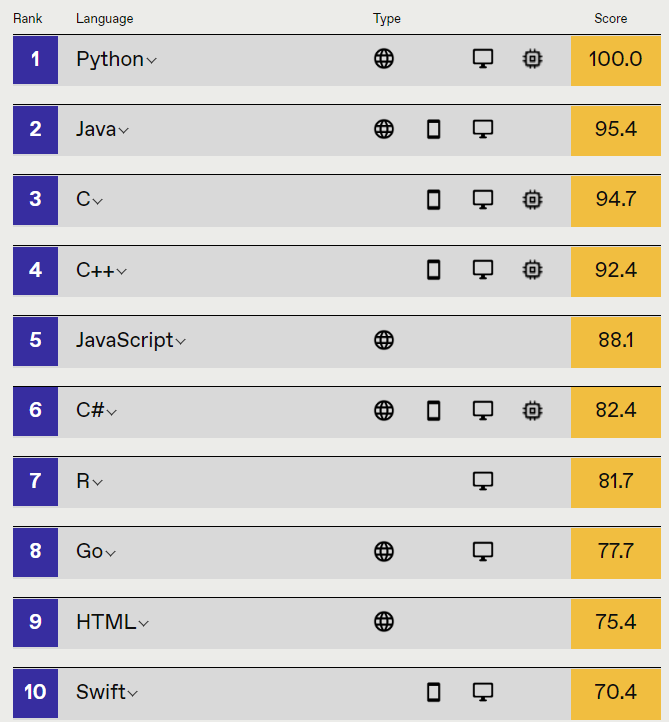
\includegraphics[width=4.6875in,height=\textheight]{images/01/toplanguage2021.png}
\caption{\url{https://spectrum.ieee.org/top-programming-languages/}}
\end{figure}

R은 데이터를 통계분석에 널리 사용되는데 이는 데이터를 눈으로 확인하기 위한 visualization 이나 벡터 연산 등의 강력한 기능 때문에 점점 더 많은 사람들이 사용하고 있습니다. 기존에는 속도나 확장성이 다른 언어들에 비해 단점으로 지적되었으나 R 언어의 계속적인 개발과 업데이트로 이러한 단점들이 빠르게 보완되고 있습니다. R 사용을 위해서는 R 언어의 코어 프로그램을 먼저 설치하고 그 다음 R 언어용 IDE(Integrated Development Environment)인 RStudio 설치가 필요합니다.


\includegraphics[width=2.60417in,height=\textheight]{images/01/rstudio.png}

Rstudio는 R 언어를 위한 오픈소스 기반 통합개발환경(IDE)으로 R 프로그래밍을 위한 편리한 기능들을 제공해 줍니다. R언어가 주목을 받고 두터운 사용자 층을 확보할 수 있게된 핵심 동력이 Rstudio 입니다. 자체적으로 최고수준의 오픈소스 개발팀이 있으며 \texttt{tidyverse}, `\texttt{,}shiny` 등의 데이터 분석 관련 주요 패키지를 개발하였고 정기적으로 conference 개최를 하면서 기술 보급의 핵심 역할을 하고 있습니다.

\begin{figure}
\centering
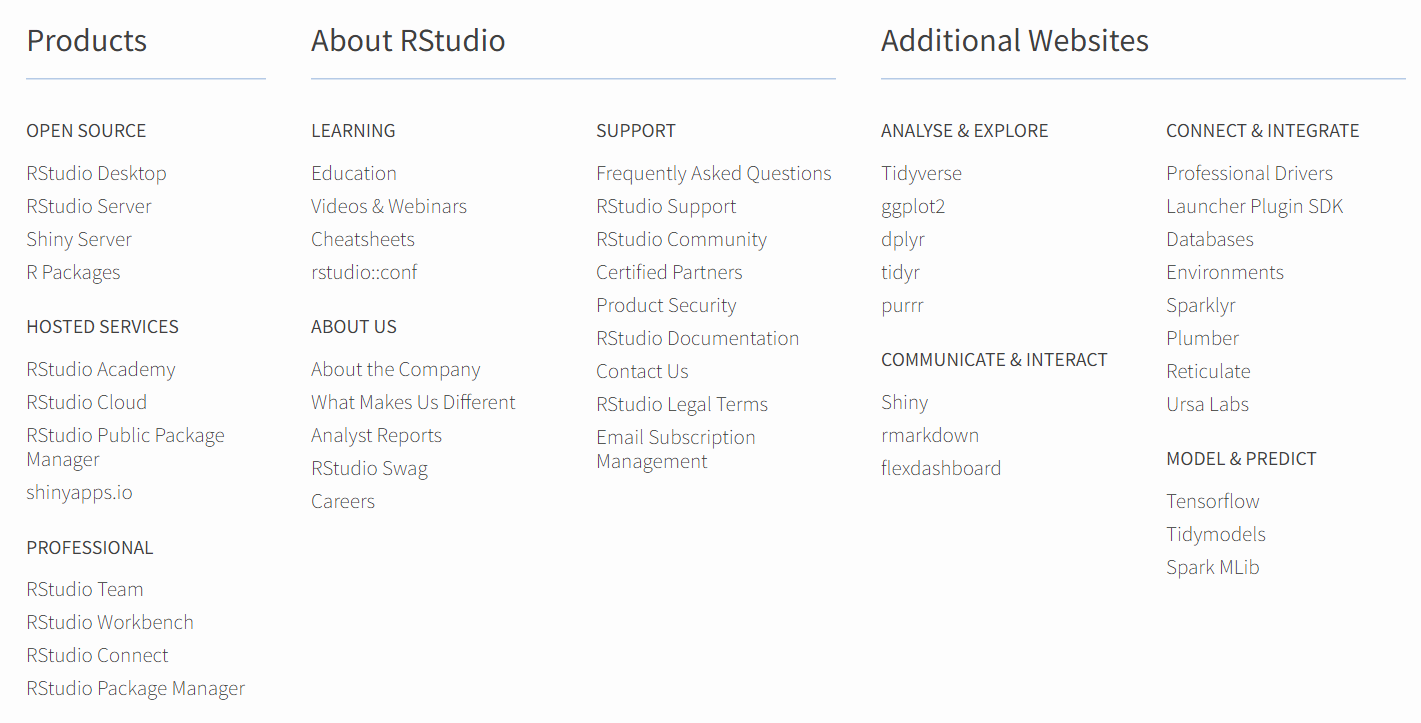
\includegraphics[width=5.72917in,height=\textheight]{images/01/rstudiobottom.png}
\caption{\url{https://www.rstudio.com/}}
\end{figure}

\hypertarget{r-rstudio-installation}{%
\section{R / Rstudio Installation}\label{r-rstudio-installation}}

\hypertarget{r-uxc124uxce58}{%
\subsection{R 설치}\label{r-uxc124uxce58}}

\begin{itemize}
\tightlist
\item
  R 사이트에 접속 후 (\url{https://www.r-project.org/}) 좌측 메뉴 상단에 위치한 CRAN 클릭.
\item
  미러 사이트 목록에서 Korea의 아무 사이트나 들어감
\item
  Download R for Windows를 클릭 후 base 링크 들어가서
\item
  Download R x.x.x for Windows 링크 클릭으로 실행 프로그램 다운로드
\item
  로컬 컴퓨터에 Download 된 R-x.x.x-win.exe 를 실행 (2022.5 현재 R 버전은 4.2.0).
\item
  설치 프로그램의 지시에 따라 R 언어 소프트웨어 설치를 완료
\end{itemize}

\hypertarget{rstudio-uxc124uxce58}{%
\subsection{Rstudio 설치}\label{rstudio-uxc124uxce58}}

\begin{itemize}
\tightlist
\item
  사이트에 접속 (\url{https://www.rstudio.com/}), 상단의 Products \textgreater{} RStudio 클릭
\item
  RStudio Desktop 선택
\item
  Download RStudio Desktop 클릭
\item
  RStudio Desktop Free 버전의 Download를 선택하고
\item
  Download RStudio for Windows 클릭, 다운로드
\item
  로컬 컴퓨터에 다운로드된 RStudio-x.x.x.exe 실행 (2022.5 현재 RStudio Desktop 2022.02.2+485)
\item
  설치 가이드에 따라 설치 완료
\end{itemize}

\hypertarget{rstudio-interface}{%
\section{Rstudio interface}\label{rstudio-interface}}

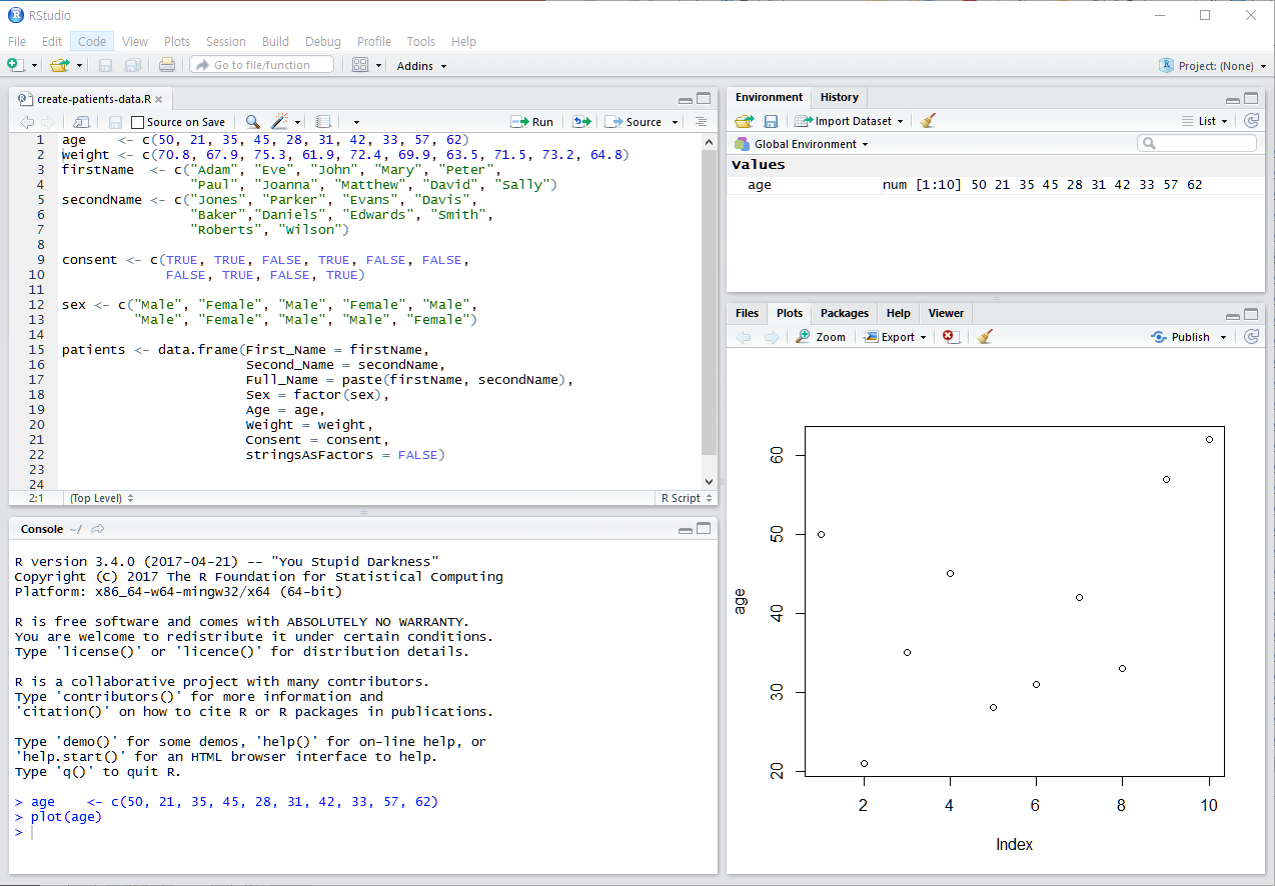
\includegraphics[width=6.25in,height=\textheight]{images/01/01-11.PNG}

\begin{itemize}
\tightlist
\item
  기본 화면에서 좌측 상단의 공간은 코드편집창, 좌측 하단은 콘솔창
\item
  각 위치를 기호에 따라서 바꿀 수 있음 (View --\textgreater{} Pane)
\end{itemize}

\hypertarget{keyboard-shortcuts}{%
\subsection{Keyboard shortcuts}\label{keyboard-shortcuts}}

\begin{itemize}
\tightlist
\item
  참고사이트

  \begin{itemize}
  \tightlist
  \item
    \url{https://support.rstudio.com/hc/en-us/articles/200711853-Keyboard-Shortcuts}
  \item
    Tools --\textgreater{} Keyboard shortcut Quick Reference (\texttt{Alt\ +\ Shift\ +\ K})
  \end{itemize}
\item
  코드편집창 이동 (\texttt{Ctrl\ +\ 1}) 콘솔창 이동(\texttt{Ctrl\ +\ 2})
\item
  한 줄 실행 (\texttt{Ctrl\ +\ Enter})
\item
  저장 (\texttt{Ctrl\ +\ S})
\item
  주석처리 (\texttt{Ctrl\ +\ Shift\ +\ C})

  \begin{itemize}
  \tightlist
  \item
    또는 \texttt{\#}으로 시작하는 라인
  \end{itemize}
\item
  텝 이동 (\texttt{Ctrl\ +\ F11}, \texttt{Ctrl\ +\ F12})
\item
  코드편집창 확대 (\texttt{Shift\ +\ Ctrl\ +\ 1}) 콘솔창 확대 (\texttt{Shift\ +\ Ctrl\ +\ 2})
\item
  컬럼 편집 (\texttt{Alt\ +\ 마우스\ 드레그})
\item
  자동 완성 기능 (Tab completion) in RStudio
\end{itemize}

\hypertarget{exercise}{%
\subsection{Exercise}\label{exercise}}

\begin{enumerate}
\def\labelenumi{\arabic{enumi}.}
\tightlist
\item
  코드편집창에서 다음을 입력/실행하고 단축키를 사용하여 주석을 넣으시오
\end{enumerate}

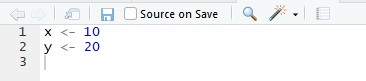
\includegraphics{images/01/01-14.PNG}

\begin{itemize}
\tightlist
\item
  단축키 \texttt{Ctrl\ +\ enter}로 코드 실행
\item
  단축키 \texttt{Ctrl\ +\ 2}로 커서 콘솔창으로 이동
\item
  \texttt{x}값 \texttt{x+y}값 확인
\item
  단축키 \texttt{Ctrl\ +\ 1}로 코드편집창 이동
\item
  단축키 \texttt{Ctrl\ +\ Shift\ +\ C} 사용
\end{itemize}

\begin{Shaded}
\begin{Highlighting}[]
\CommentTok{\# x \textless{}{-} 10}
\CommentTok{\# y \textless{}{-} 20}
\end{Highlighting}
\end{Shaded}

\hypertarget{environment-and-files}{%
\subsection{Environment and Files}\label{environment-and-files}}

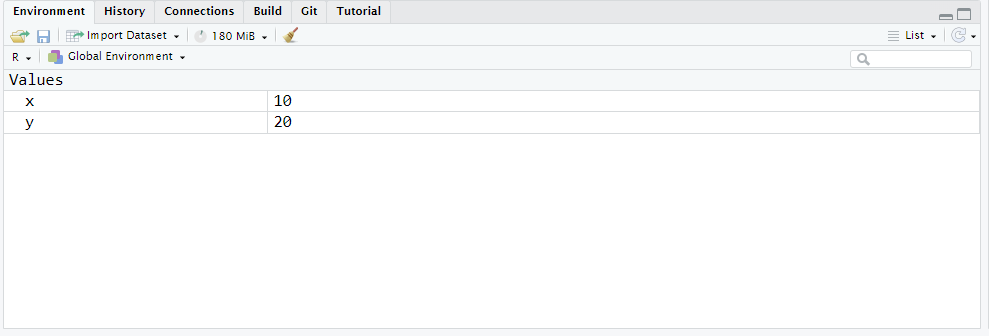
\includegraphics{images/01/envandhist.png}

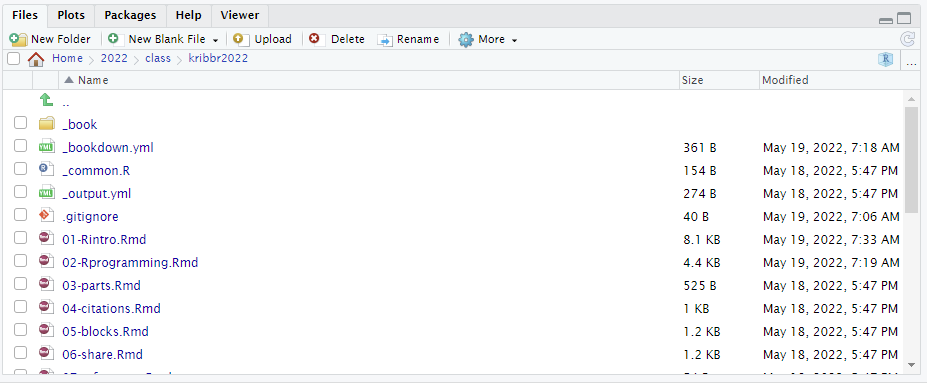
\includegraphics{images/01/fileandpackages.png}

\hypertarget{start-a-project}{%
\section{Start a project}\label{start-a-project}}

프로젝트를 만들어서 사용할 경우 파일이나 디렉토리, 내용 등을 쉽게 구분하여 사용 가능합니다. 아래와 같이 임의의 디렉토리에 \texttt{kribbR} 이라는 디렉토리를 생성하고 \texttt{lecture1} 프로젝트를 만듭니다.

\begin{quote}
File \textgreater{} New Project \textgreater{} New Directory \textgreater{} New Project \textgreater{} ``kribbR'' \textgreater{} Create Project
\end{quote}

시작할 때는 해당 디렉토리의 \texttt{xxx.Rproj} 파일을 클릭합니다. Rstudio 오른쪽 상단 프로젝트 선택을 통해서 빠르게 다른 프로젝트의 작업공간으로 이동할 수 있습니다.

\hypertarget{hello-world}{%
\subsection{Hello world}\label{hello-world}}

\begin{quote}
File \textgreater{} New File \textgreater{} R markdown \textgreater{} OK
\end{quote}

\begin{Shaded}
\begin{Highlighting}[]
\NormalTok{mystring }\OtherTok{\textless{}{-}} \StringTok{"Hello }\SpecialCharTok{\textbackslash{}n}\StringTok{ world!"}
\FunctionTok{cat}\NormalTok{(mystring)}
\FunctionTok{print}\NormalTok{(mystring)}
\end{Highlighting}
\end{Shaded}

\hypertarget{getting-help}{%
\section{Getting help}\label{getting-help}}

R은 방대한 양의 도움말 데이터를 제공하며 다음과 같은 명령어로 특정 함수의 도움말과 예제를 찾아볼 수 있습니다. \texttt{?} 명령을 사용하면 되며 구글이나 웹에서도 도움을 얻을 수 있습니다.

\begin{Shaded}
\begin{Highlighting}[]
\FunctionTok{help}\NormalTok{(}\StringTok{"mean"}\NormalTok{)}
\NormalTok{?mean}
\FunctionTok{example}\NormalTok{(}\StringTok{"mean"}\NormalTok{)}
\FunctionTok{help.search}\NormalTok{(}\StringTok{"mean"}\NormalTok{)}
\NormalTok{??mean}
\FunctionTok{help}\NormalTok{(}\AttributeTok{package=}\StringTok{"MASS"}\NormalTok{)}
\end{Highlighting}
\end{Shaded}

또한 \url{https://www.rstudio.com/resources/cheatsheets/} 에서는 다양한 R언어의 기능을 한 눈에 알아볼 수 있게 만든 cheatsheet 형태의 문서를 참고할 수 있습니다.

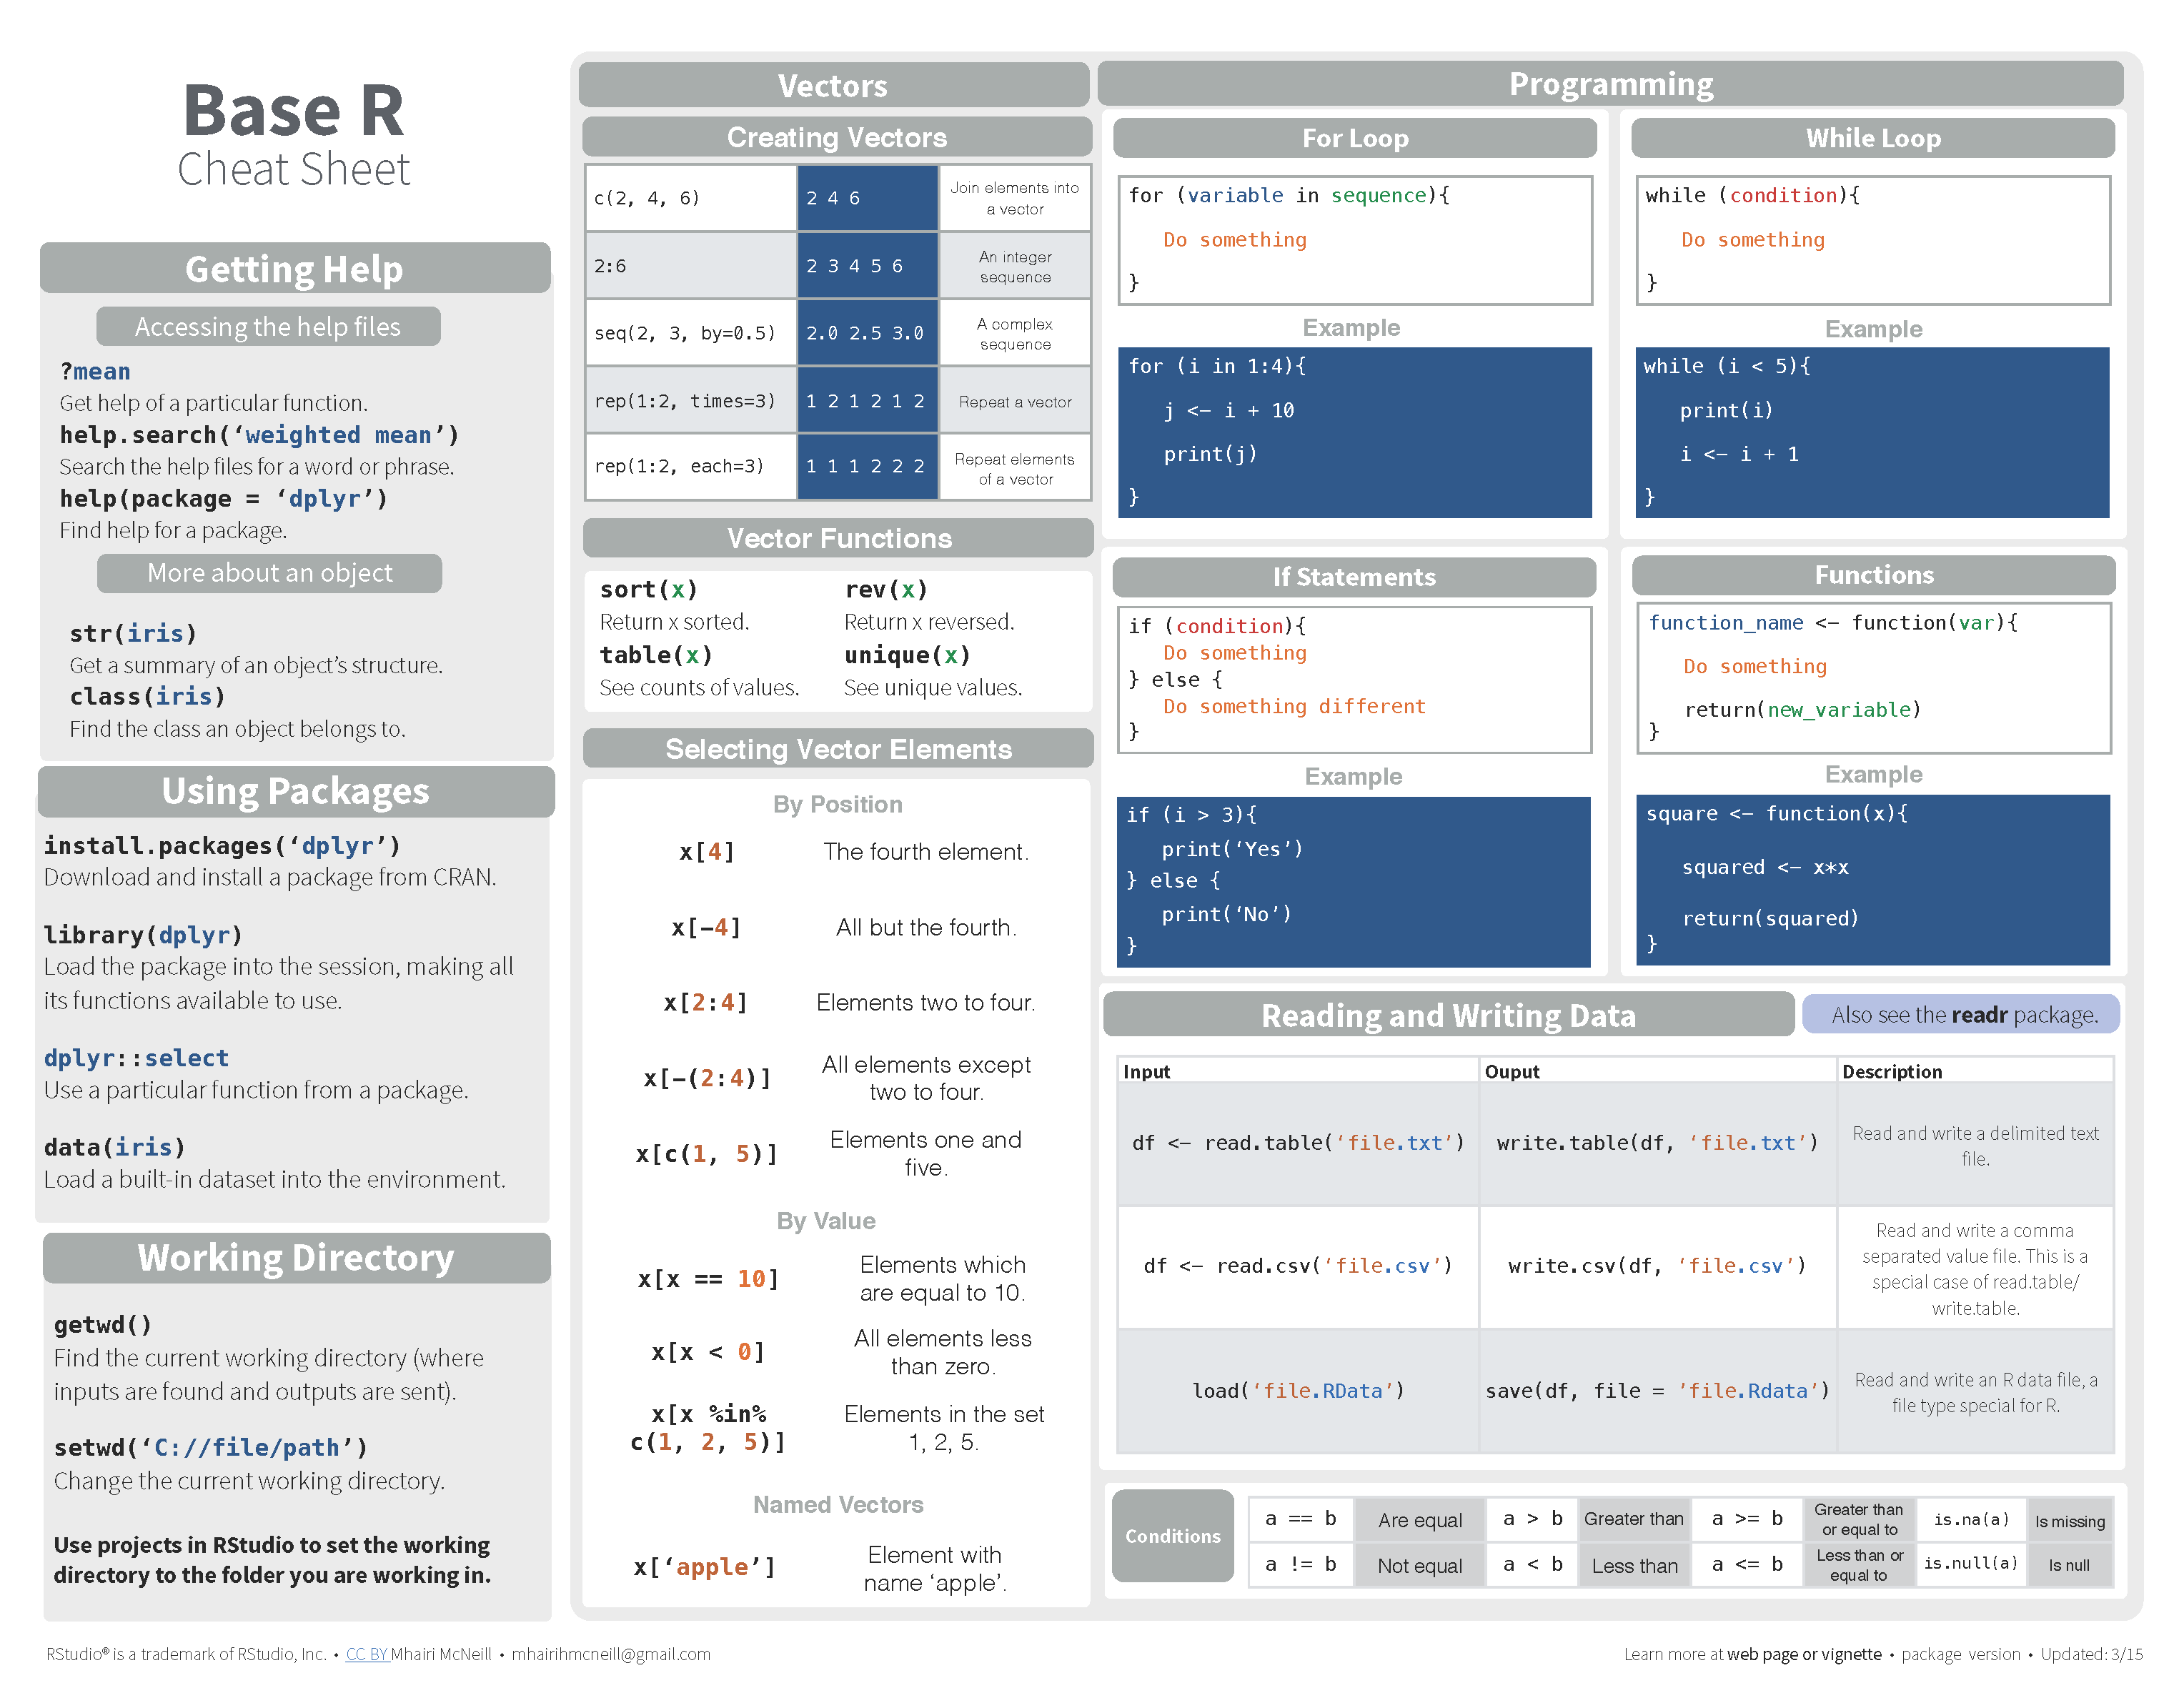
\includegraphics[width=5.72917in,height=\textheight]{images/01/base-r_1.png}
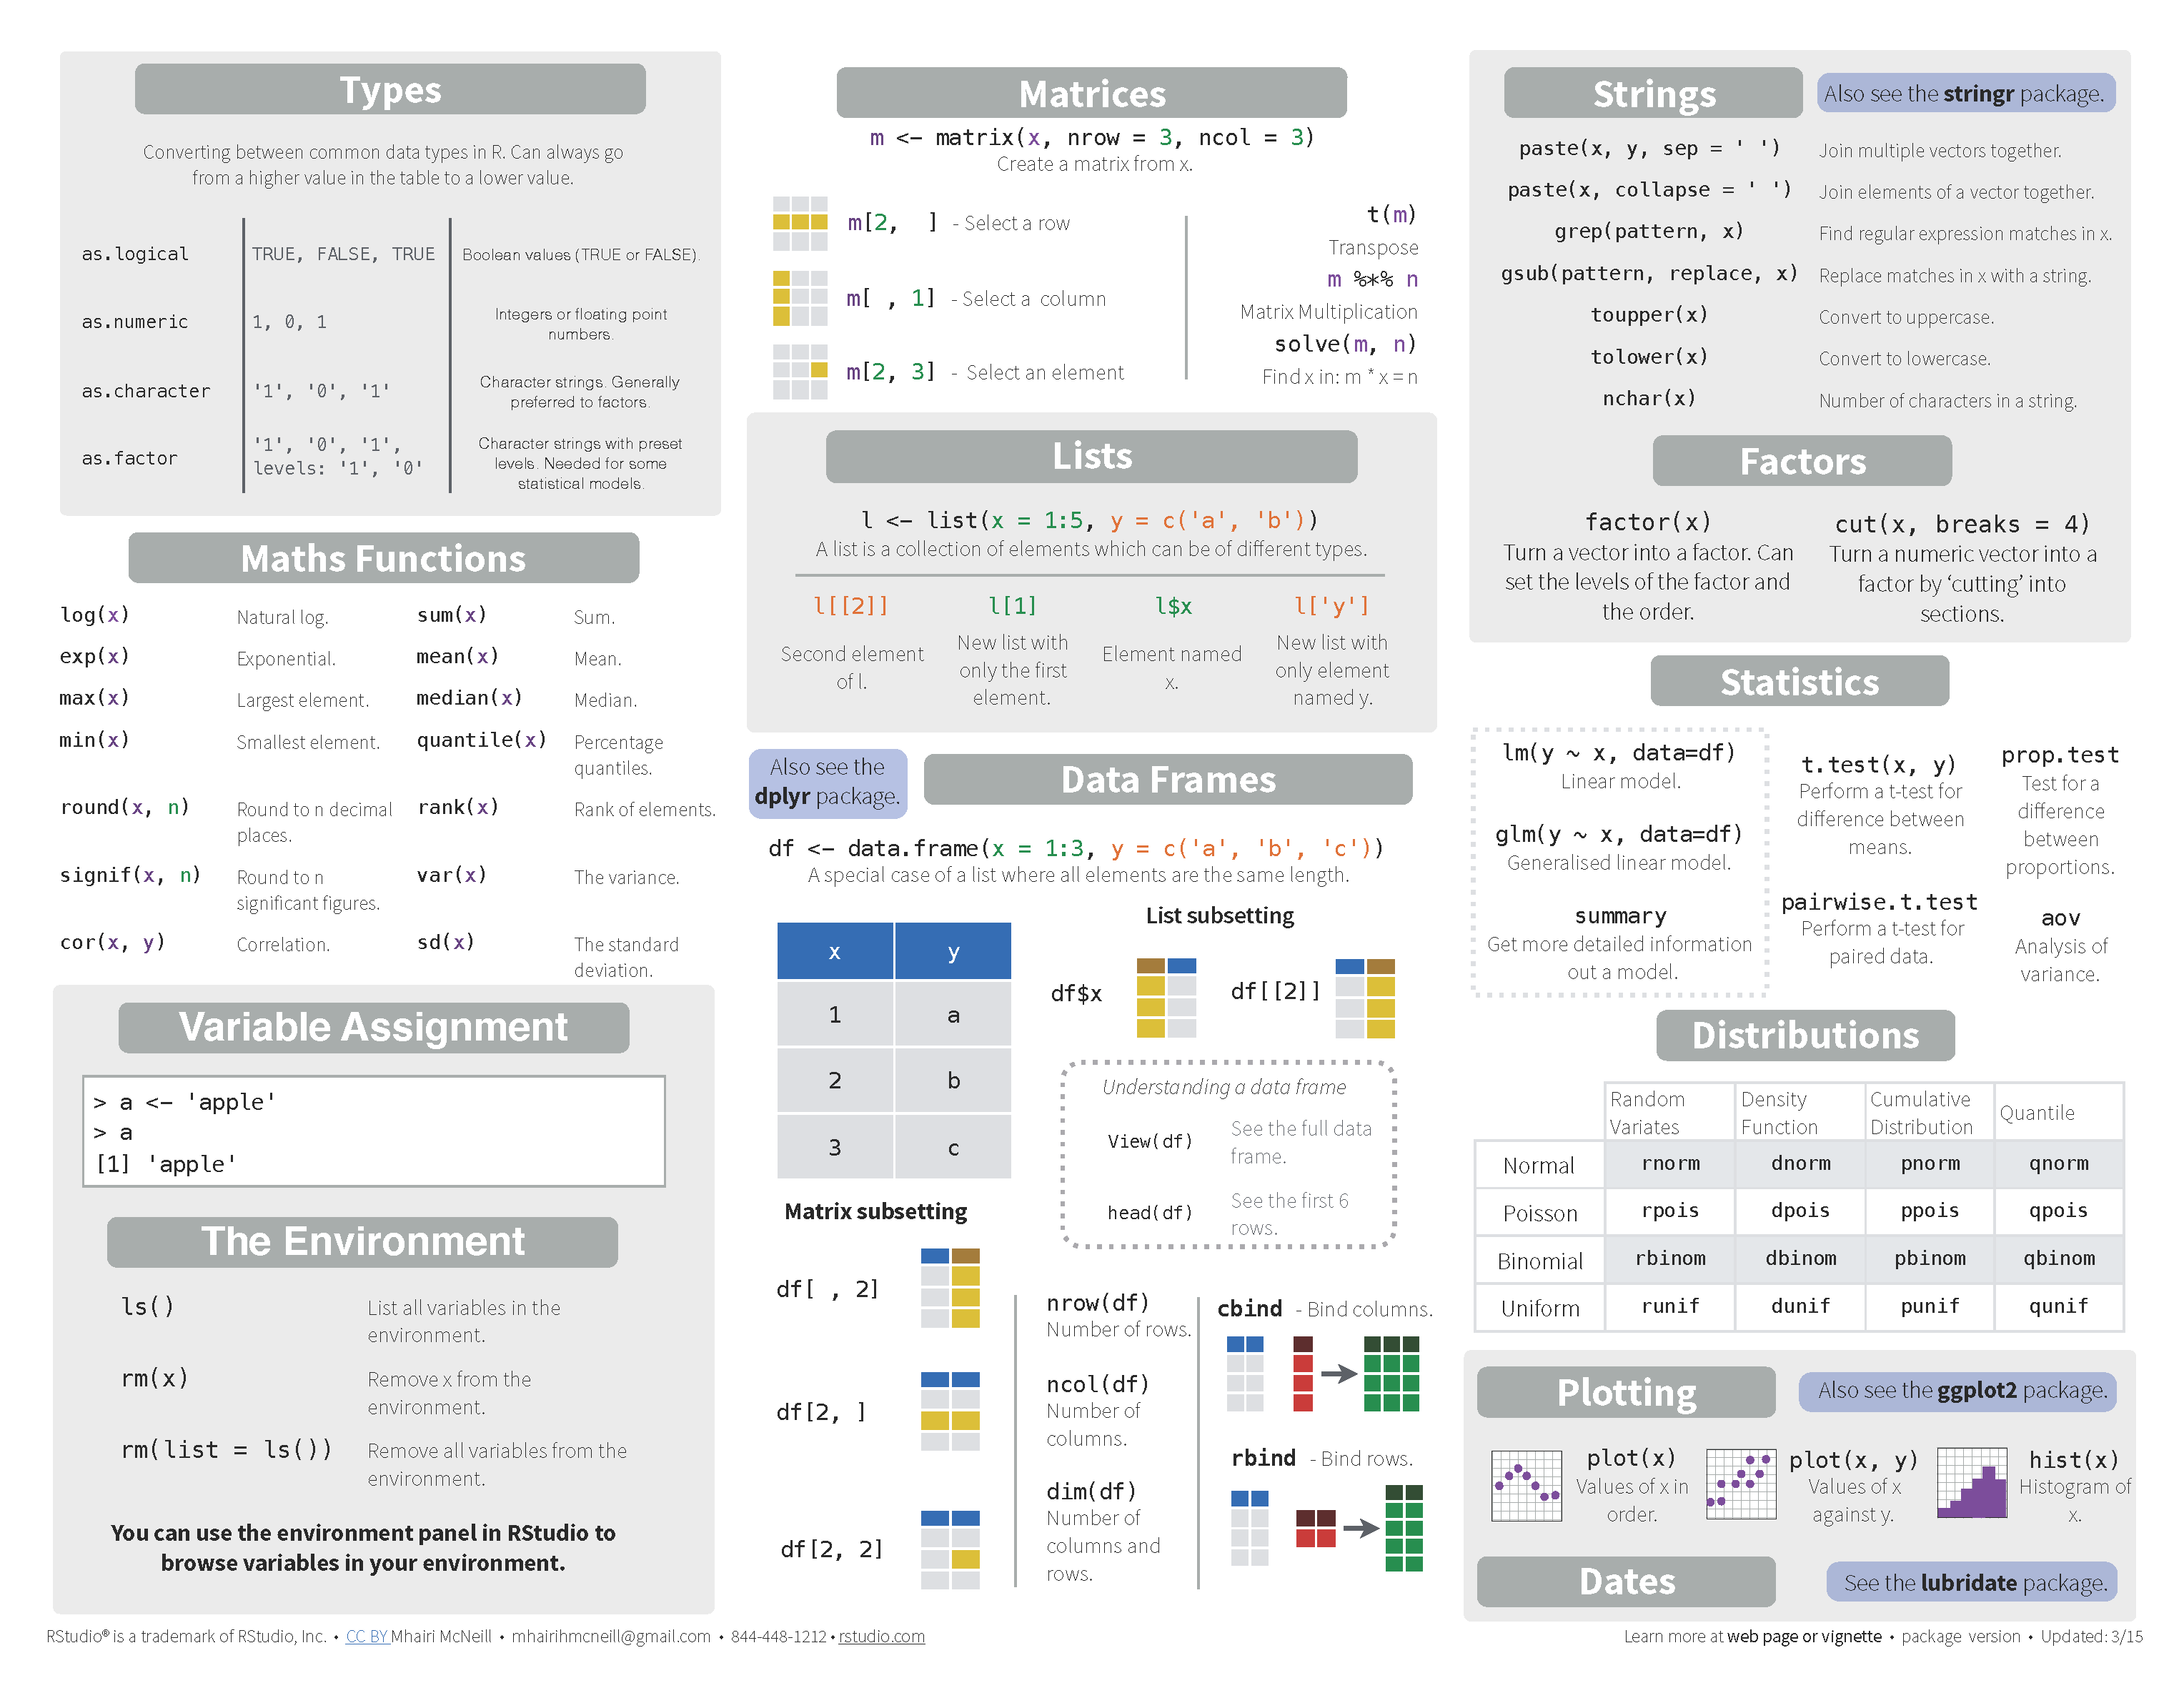
\includegraphics[width=56.77083in,height=\textheight]{images/01/base-r_2.png}

\hypertarget{r-packages-and-dataset}{%
\section{R packages and Dataset}\label{r-packages-and-dataset}}

R 패키지는 함수와 데이터셋의 묶음으로 다른 사람들이 만들어 놓은 코드나 기능을 가져와서 사용하므로써 코드 작성의 수고로움을 줄이고 편리하고 검증된 함수(기능)를 빠르게 도입하여 사용할 수 있다는 장점이 있습니다. 예를 들어 \texttt{sd()} 함수는 \texttt{stats} package에서 제공하는 함수로써 표준편차 계산을 위한 별도의 함수를 만들어서 사용할 필요가 없이 바로 (stats 패키지는 R 기본 패키지로) 별도 설치 없이 바로 사용 가능합니다.

이러한 패키지는 인터넷의 \texttt{repository}에서 구할 수 있으며 대표적인 \texttt{repository}는 The Comprehensive R Archive Network (CRAN) (\url{http://cran.r-project.org/web/views/}) 와 생물학자를 위한 Bioconductor (\url{http://www.bioconductor.org/}) 가 있습니다. 이러한 패키지의 설치는 아래와 같이 RStudio를 이용하거나 콘솔창에서 \texttt{install.packages()} 함수를 이용할 수 있습니다.

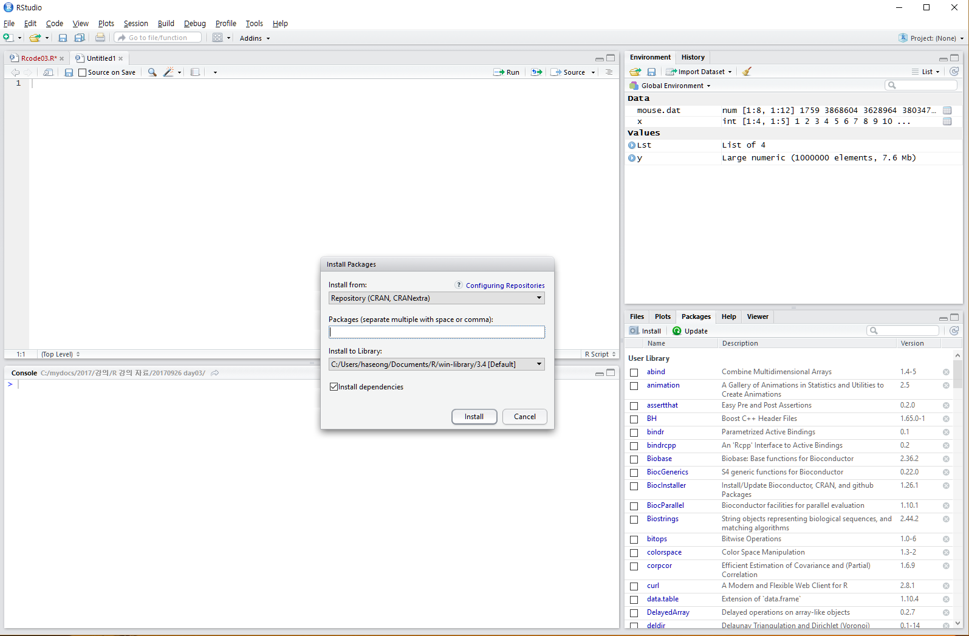
\includegraphics[width=5.72917in,height=\textheight]{images/01/01-18.PNG}

패키지를 설치하고 사용하기 위해서는 \texttt{library()} 함수를 사용해서 관련 명령어를 사용하기 전에 미리 loading 해 두어야 합니다. 한 번 로딩으로 작업 세션이 끝날때까지 관련된 함수를 사용할 수 있으나 R 세션이나 RStudio를 재시작 할 경우 다시 로딩해야 사용할 수 있습니다.

\begin{Shaded}
\begin{Highlighting}[]
\FunctionTok{library}\NormalTok{(UsingR)}
\end{Highlighting}
\end{Shaded}

\begin{itemize}
\tightlist
\item
  R 설치 디렉토리
\item
  R 패키지 설치 디렉토리
\end{itemize}

\begin{Shaded}
\begin{Highlighting}[]
\FunctionTok{.libPaths}\NormalTok{()}
\FunctionTok{path.package}\NormalTok{()}
\end{Highlighting}
\end{Shaded}

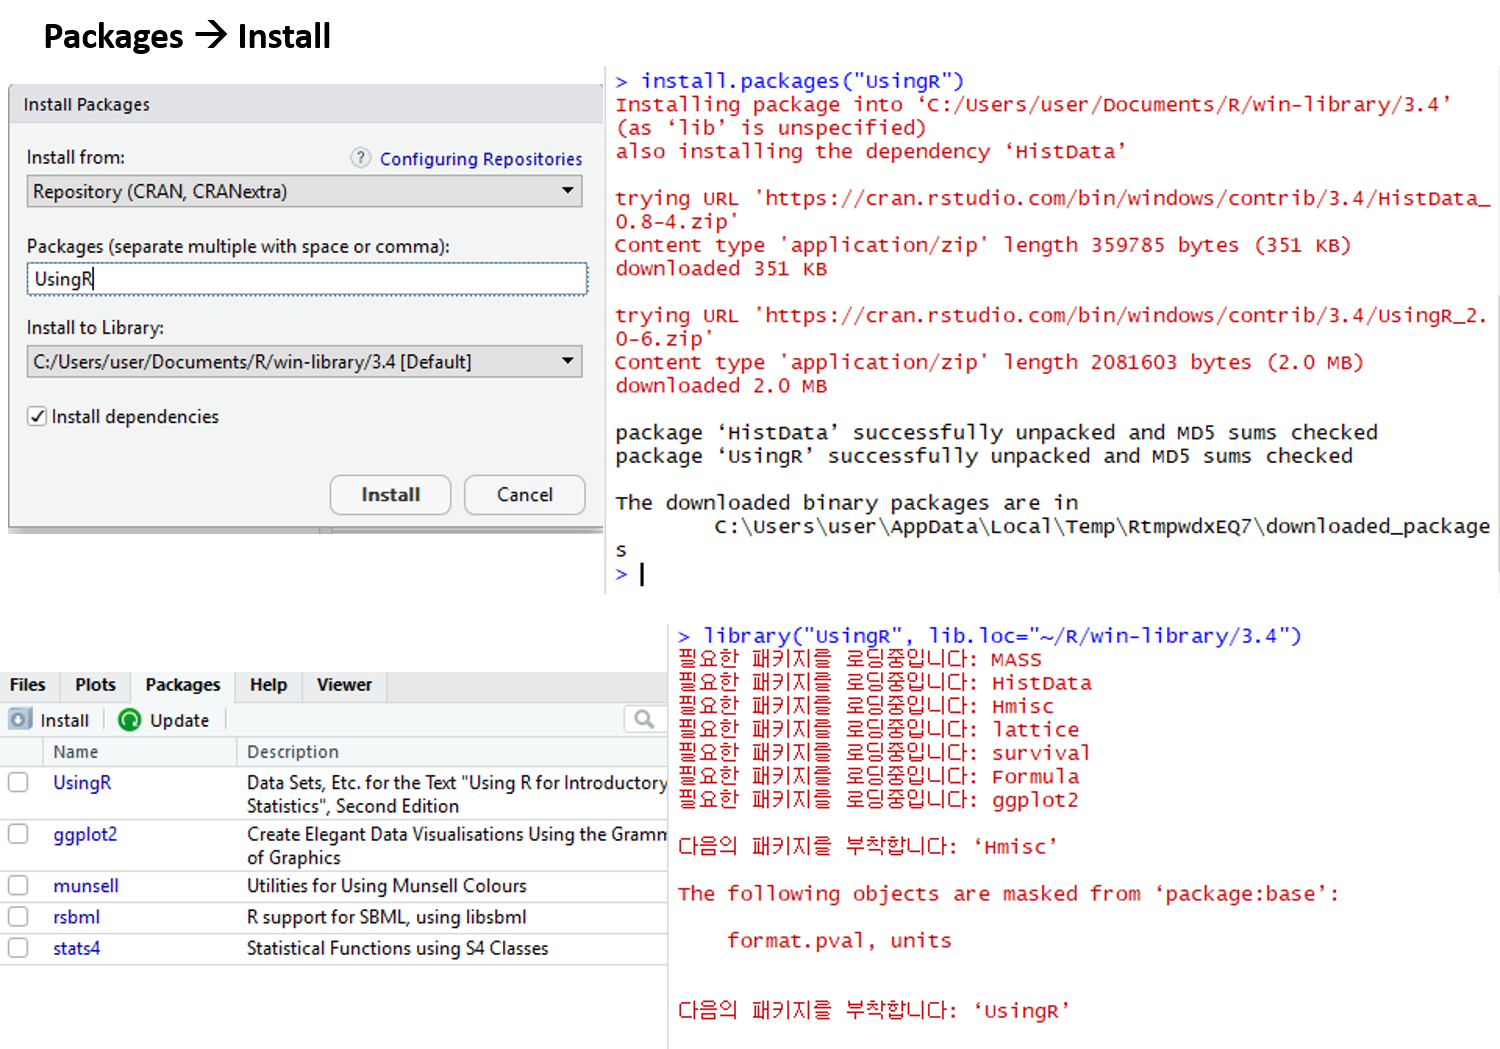
\includegraphics[width=6.25in,height=\textheight]{images/01/01-19.PNG}

일반적으로 패키지 안에 관련된 데이터도 같이 저장되어 있으며 \texttt{data()} 함수를 이용해서 패키지 데이터를 사용자 작업공간에 복사해서 사용 가능합니다.

\begin{Shaded}
\begin{Highlighting}[]
\FunctionTok{head}\NormalTok{(rivers)}
\FunctionTok{length}\NormalTok{(rivers)}
\FunctionTok{class}\NormalTok{(rivers)}
\FunctionTok{data}\NormalTok{(rivers)}
\FunctionTok{data}\NormalTok{(}\AttributeTok{package=}\StringTok{"UsingR"}\NormalTok{)}
\FunctionTok{library}\NormalTok{(HistData)}
\FunctionTok{head}\NormalTok{(Cavendish)}
\FunctionTok{str}\NormalTok{(Cavendish)}
\FunctionTok{head}\NormalTok{(Cavendish}\SpecialCharTok{$}\NormalTok{density2)}
\end{Highlighting}
\end{Shaded}

\begin{center}\rule{0.5\linewidth}{0.5pt}\end{center}

이 저작물은 크리에이티브 커먼즈 저작자표시-비영리-변경금지 4.0 국제 라이선스에 따라 이용할 수 있습니다.

\hypertarget{rmarkdown}{%
\chapter{Rmarkdown}\label{rmarkdown}}

R markdown은 데이터를 분석하는 코드와 리포트를 동시에 수행할 수 있는 일종의 통합 문서입니다. 워드나 아래한글에서 프로그래밍과 데이터분석을 위한 코드를 작성할 수 있는 경우라고 생각해도 됩니다. Plain-text 기반의 markdown 문법을 사용하며 R markdown으로 작성된 문서는 HTML, PDF, MS word, Beamer, HTML5 slides, books, website 등 다양한 포멧의 출력물로 변환할 수 있습니다.

\begin{figure}
\centering
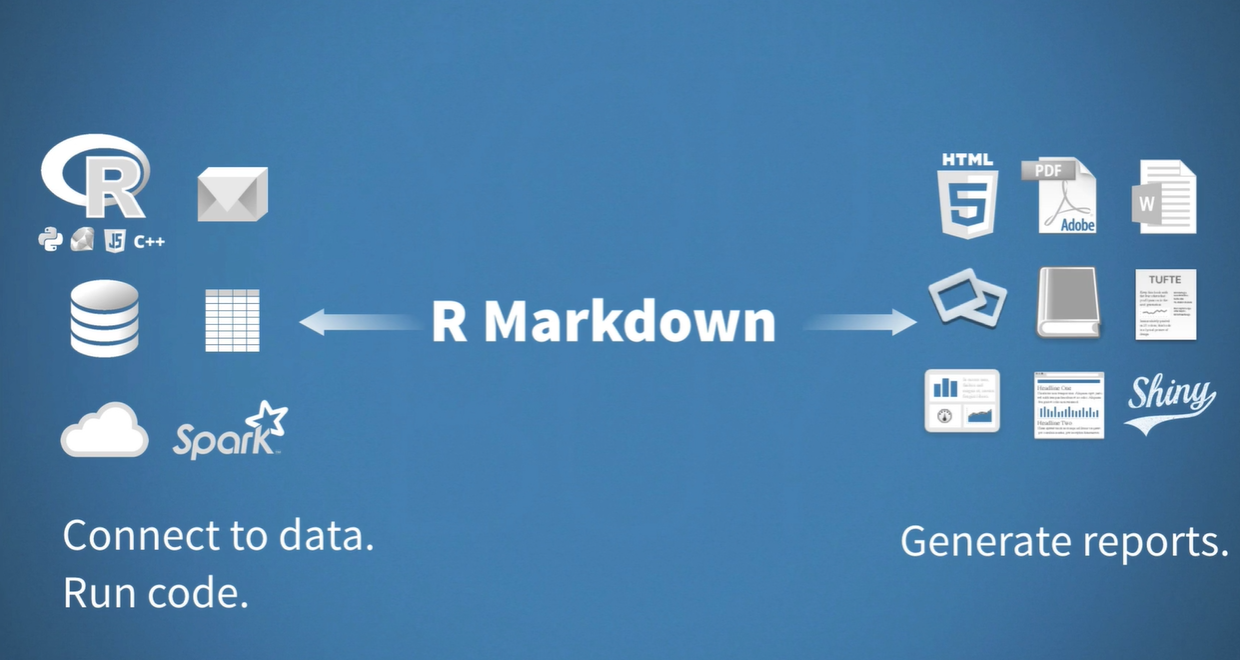
\includegraphics{images/rmarkdown/rmarkdown-01.PNG}
\caption{Image from rmarkdown.rstudio.com}
\end{figure}

Rmarkdown 웹사이트에 R markdown 소개 동영상과 \href{https://rmarkdown.rstudio.com/lesson-1.html}{R markdown 공식 사이트 메뉴얼} 관련 서적 \href{https://bookdown.org/yihui/rmarkdown/}{R markdown: The Definitive Guide}를 참고하세요. 또한 R markdown을 사용할 때 \href{https://github.com/rstudio/cheatsheets/raw/master/rmarkdown-2.0.pdf}{cheatsheet}를 옆에 두고 수시로 보면서 사용하시면 많은 도움이 될 수 있습니다.

\hypertarget{r-markdownuxc758-uxae30uxbcf8-uxc791uxb3d9-uxc6d0uxb9ac}{%
\section{R markdown의 기본 작동 원리}\label{r-markdownuxc758-uxae30uxbcf8-uxc791uxb3d9-uxc6d0uxb9ac}}

R markdown은 plain text 기반으로 작성되며 Rmd 라는 확장자를 갖는 파일로 저장됩니다. 다음과 같은 텍스트 파일이 Rmd 파일의 전형적인 예 입니다.

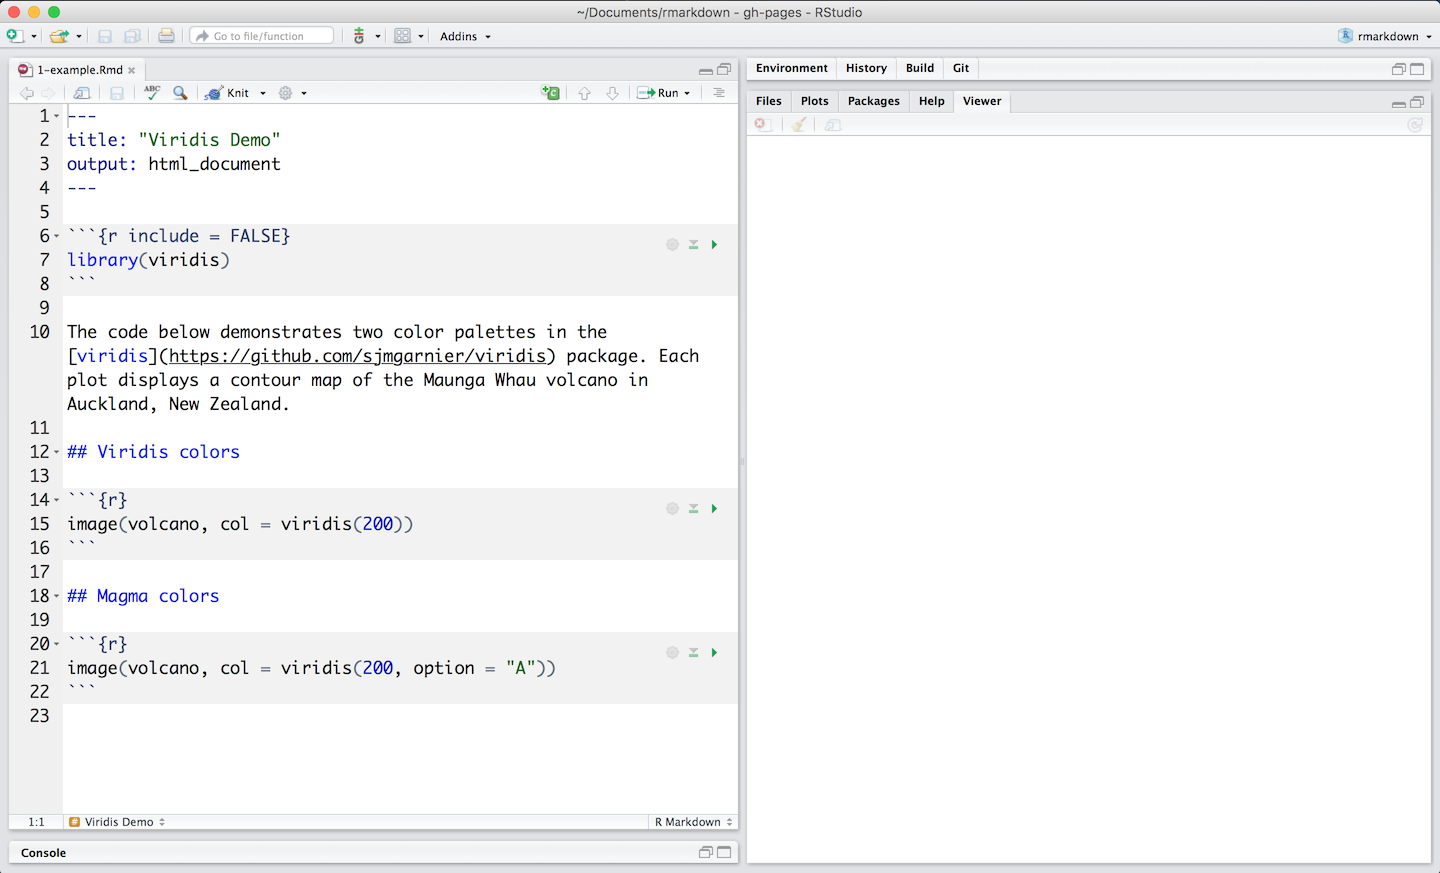
\includegraphics[width=5.72917in,height=\textheight]{images/rmarkdown/how-1-file.png}

위 예제에서 네 가지 다른 종류의 컨텐츠를 볼 수 있습니다. 하나는 - - - 으로 둘러쌓인 내용으로 YAML 이라고 하며 JSON과 같은 데이터 직렬화를 수행하는 하나의 데이터 저장 포멧입니다. 백틱(`) 으로 둘러쌓인 코드청그(Code Chunks)라고 하는 부분에는 R이나 python 등의 다양한 코드(실재 작동하는)를 넣어서 사용합니다. 그리고 \#\#\# 으로 표시된 글은 제목 글을 나타내며 나머지는 일반적인 텍스트를 나타냅니다.

이러한 R markdown 파일은 \texttt{render}라는 명령어로 원하는 포맷의 문서로 변환할 수 있습니다. 다음 예의 파일을 pdf 형식으로 rendering 하기 위해서는 YAML에 pdf 임을 명시하고 아래와 같이 \texttt{render}함수를 사용하면 됩니다. 또는 Rstudio 코드 입력창 상단의 Knit 버튼으로 pdf나 html 문서를 생성할 수 있습니다.

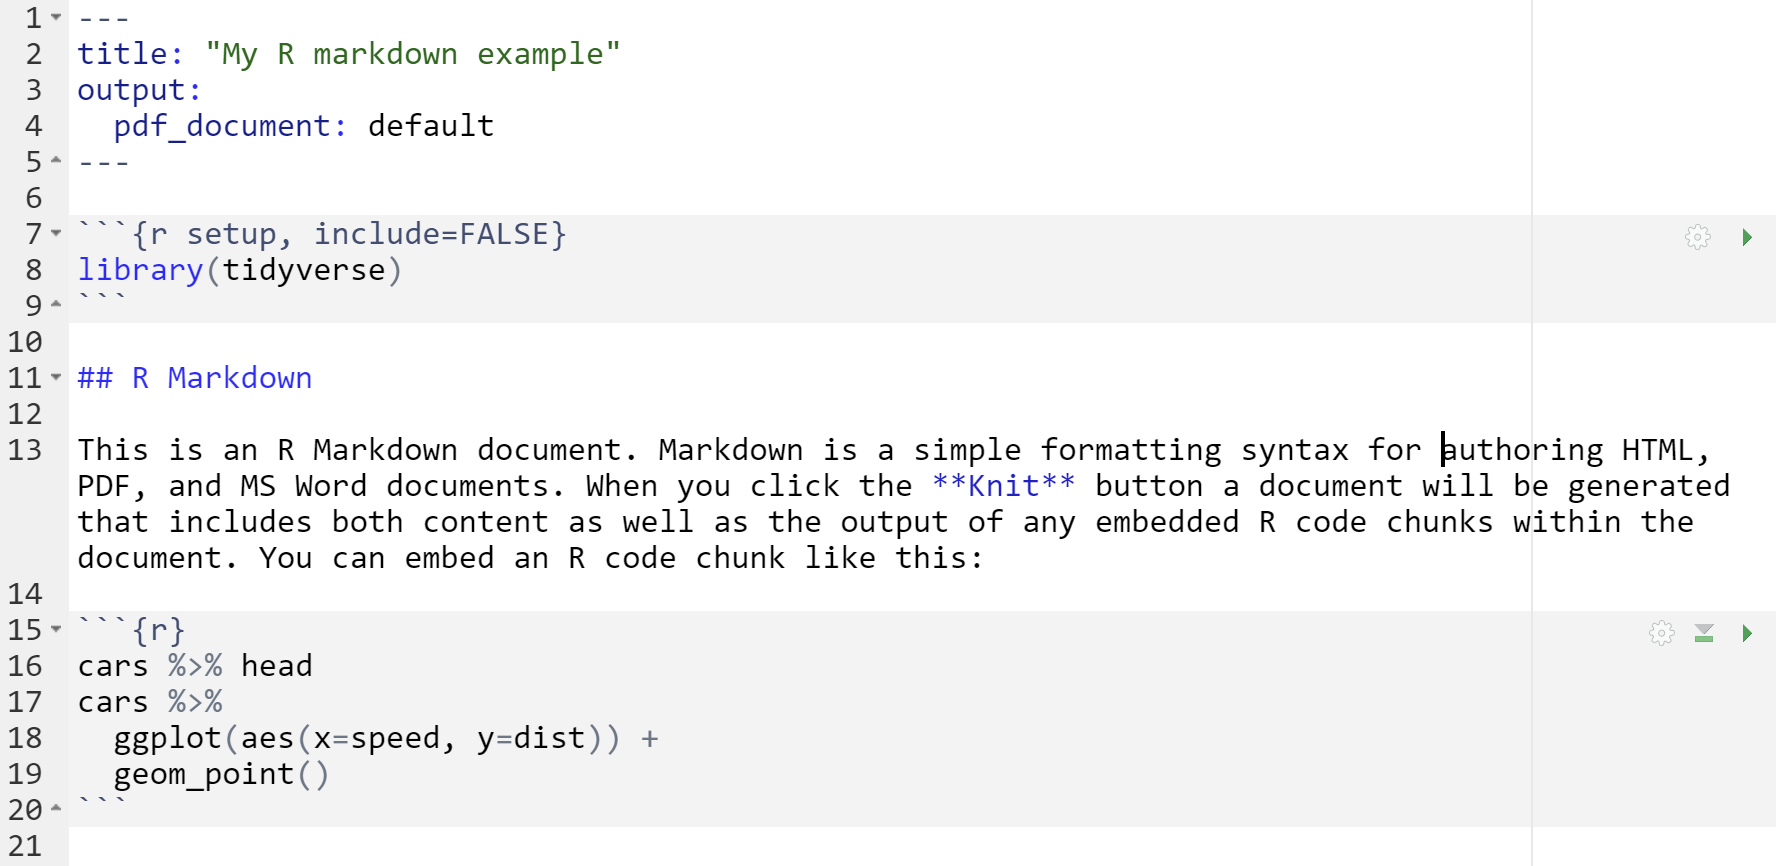
\includegraphics[width=5.72917in,height=\textheight]{images/rmarkdown/example2.PNG}

\begin{Shaded}
\begin{Highlighting}[]
\FunctionTok{render}\NormalTok{(}\StringTok{"examples/test.Rmd"}\NormalTok{, }\AttributeTok{output\_format =} \StringTok{"pdf\_document"}\NormalTok{)}
\end{Highlighting}
\end{Shaded}

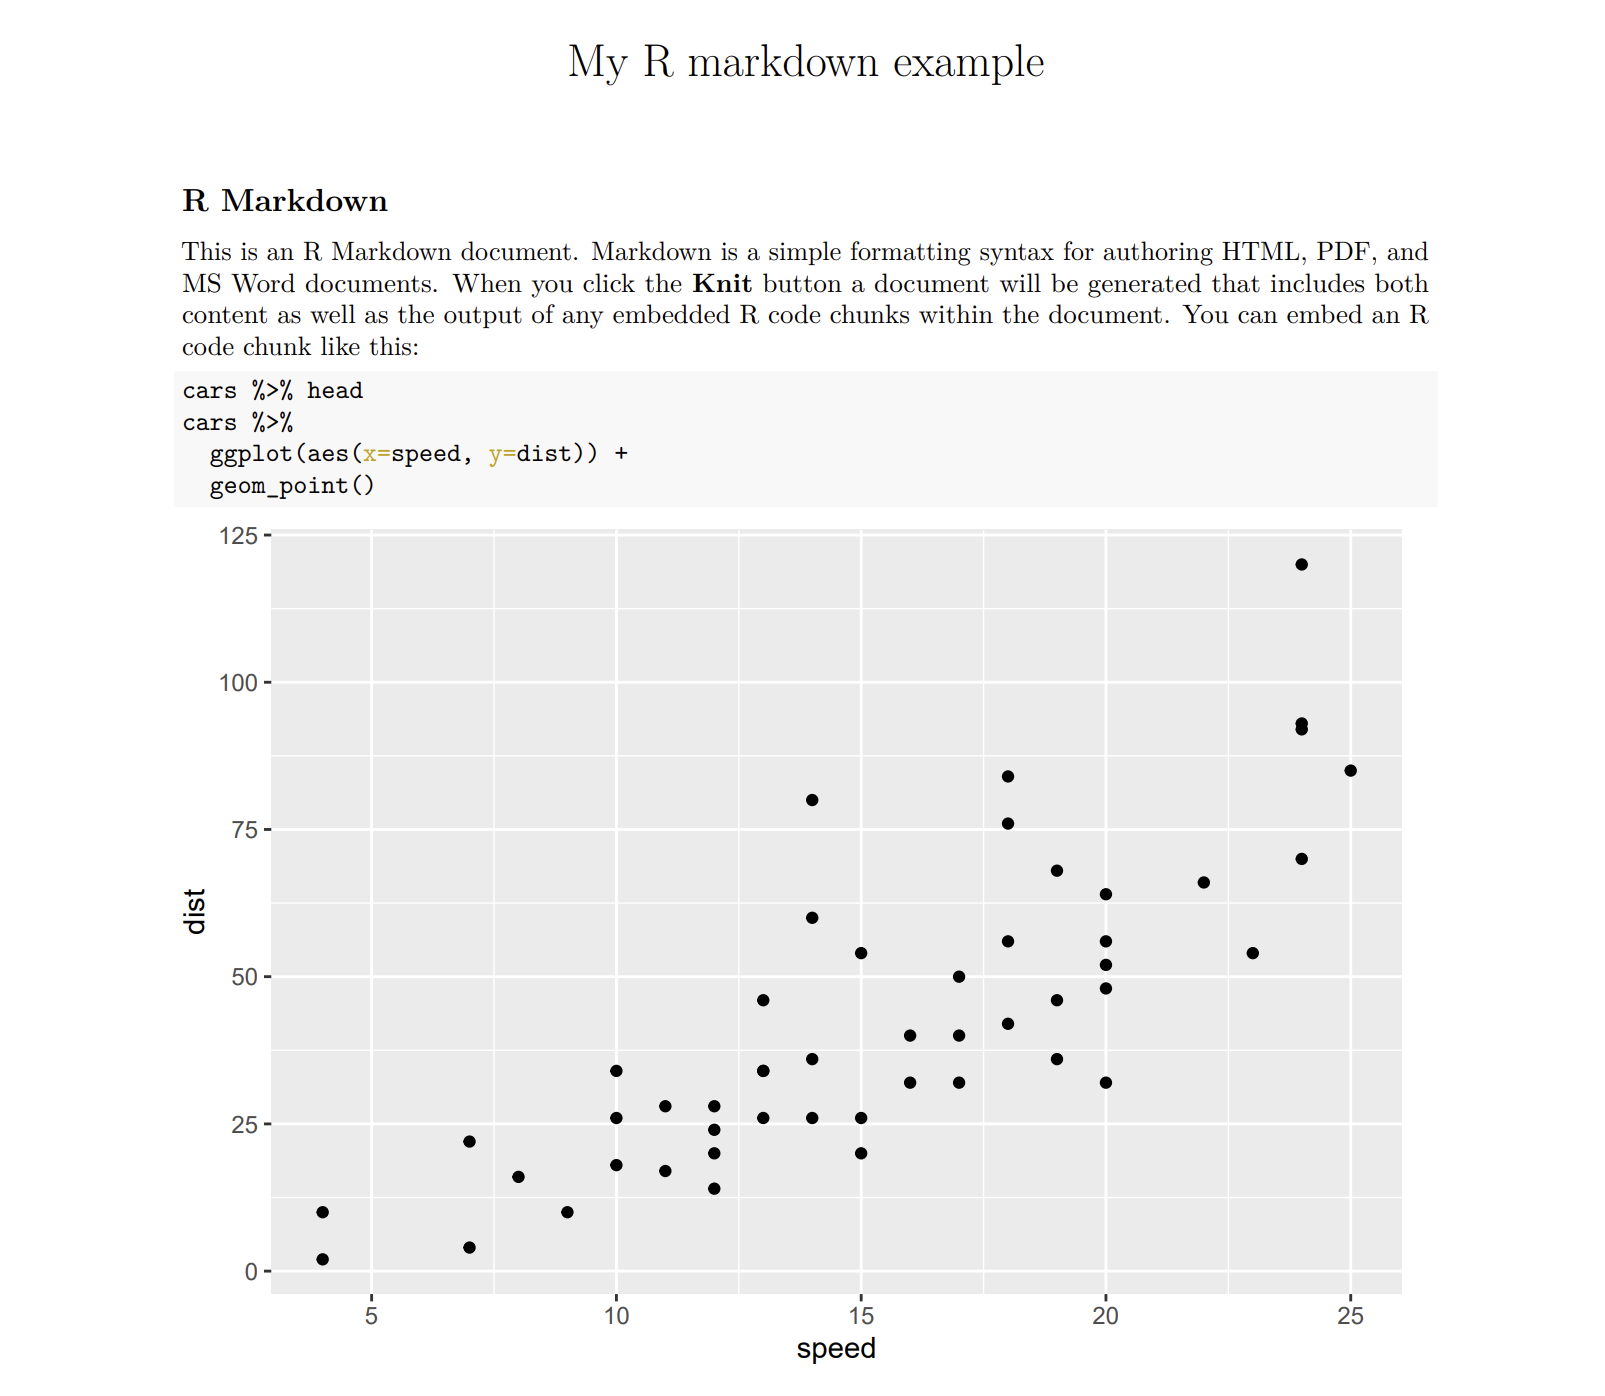
\includegraphics[width=5.72917in,height=\textheight]{images/rmarkdown/ex_pdf.PNG}

R markdown의 작동 원리는 Rmd 파일을 만든 후 \texttt{render} 함수를 부르면 \href{https://yihui.org/knitr/}{knitr} 소프트웨어가 R 코드를 실행시킨 후 markdown (.md) 파일을 생성합니다. 이 후 .md 파일을 \href{https://pandoc.org/}{pandoc} 이라는 문서변환기가 원하는 문서 형태로 전환해 줍니다.

\hypertarget{uxcf54uxb4dc-uxc785uxb825}{%
\section{코드 입력}\label{uxcf54uxb4dc-uxc785uxb825}}

R markdown에서 사용하는 코드청크는 CTRL+ALT+I 단축키를 사용해서 넣을 수 있으며 다음과 같은 몇 가지 옵션으로 코드 스니펫들의 실행/숨김 여부를 결정할 수 있습니다.

\begin{itemize}
\tightlist
\item
  \texttt{include\ =\ FALSE} : 코드는 실행되지만 보고서에 결과와 코드가 보여지지 않음
\item
  \texttt{echo\ =\ FALSE} : 코드는 실행되고 보고서에 결과가 포함되지만 코드는 보여지지 않음
\item
  \texttt{eval\ =\ FALSE} : 코드가 실행되지 않지만 보고서에 코드는 보여짐
\item
  \texttt{message\ =\ FALSE}, \texttt{warning=FALSE}, \texttt{error=FALSE} : 코드에 의해서 발생되는 메세지/경고/에러가 보고서에 보여지지 않음
\item
  \texttt{fig.cap\ =\ "..."} : 코드로 그려지는 그래프에 캡션을 붙일 수 있음
\end{itemize}

\begin{figure}
\centering
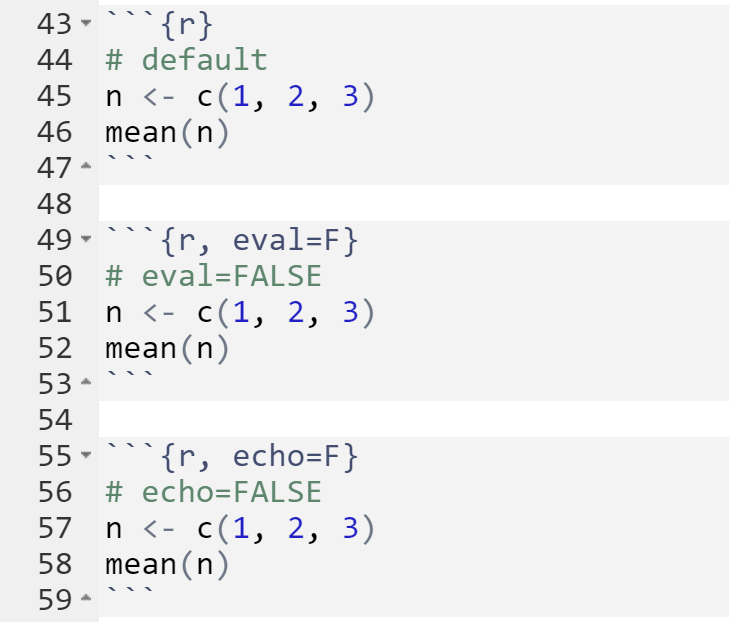
\includegraphics[width=3.125in,height=\textheight]{images/rmarkdown/codechunk1.PNG}
\caption{코드청크 옵션 예시}
\end{figure}

\begin{Shaded}
\begin{Highlighting}[]
\CommentTok{\# default}
\NormalTok{n }\OtherTok{\textless{}{-}} \FunctionTok{c}\NormalTok{(}\DecValTok{1}\NormalTok{, }\DecValTok{2}\NormalTok{, }\DecValTok{3}\NormalTok{)}
\FunctionTok{mean}\NormalTok{(n)}
\CommentTok{\#\textgreater{} [1] 2}
\end{Highlighting}
\end{Shaded}

\begin{Shaded}
\begin{Highlighting}[]
\CommentTok{\# eval=FALSE}
\NormalTok{n }\OtherTok{\textless{}{-}} \FunctionTok{c}\NormalTok{(}\DecValTok{1}\NormalTok{, }\DecValTok{2}\NormalTok{, }\DecValTok{3}\NormalTok{)}
\FunctionTok{mean}\NormalTok{(n)}
\end{Highlighting}
\end{Shaded}

\begin{verbatim}
#> [1] 2
\end{verbatim}

R markdown에서는 \texttt{r} 을 사용해서 코드청크가 아닌 곳에 R 코드를 넣을 수 있습니다. 예를 들어 n은 1, 2, 3 값을 가지는 벡터 입니다. 또한 R 언어 외에도 \texttt{Python}, \texttt{SQL}, \texttt{Bash}, \texttt{Rcpp}, \texttt{Stan}, \texttt{JavaScript}, \texttt{CSS} 등의 다양한 프로그래밍 언어에 대해서도 지원합니다. 그런데 이러한 언어들이 사용 가능해지기 위해서는 해당 언어들을 실행해주는 엔진이 있어야 하며 python의 경우 \texttt{reticulate} 라는 패키지가 이러한 기능을 담당합니다. 이 패키지를 설치할 경우 miniconda라는 가상환경 및 데이터 분석을 위한 오픈소스 패키지가 자동으로 설치됩니다.

\begin{Shaded}
\begin{Highlighting}[]
\NormalTok{x }\OperatorTok{=} \StringTok{"hello, python in R"}
\BuiltInTok{print}\NormalTok{(x.split(}\StringTok{\textquotesingle{} \textquotesingle{}}\NormalTok{))}
\end{Highlighting}
\end{Shaded}

\hypertarget{markdown-uxbb38uxbc95}{%
\section{Markdown 문법}\label{markdown-uxbb38uxbc95}}

마크다운은 plain text 기반의 마크업 언어로서 마크업 언어는 태그 등을 이용해서 문서의 데이터 구조를 명시하는데 이러한 태그를 사용하는 방법 체계를 마크업 언어라고 합니다. 가장 대표적으로 html 이 있습니다.

\begin{verbatim}
<html>
  <head>
    <title> Hello HTML </title>
  </head>
  <body>
  Hello markup world!
  </body>
</html>
\end{verbatim}

마크다운도 몇 가지 태그를 이용해서 문서의 구조를 정의하고 있으며 상세한 내용은 \href{https://rmarkdown.rstudio.com/authoring_pandoc_markdown.html}{Pandoc 마크다운 문서}를 참고하시기 바랍니다. 마크다운언어의 철학은 쉽게 읽고 쓸 수 있는 문서입니다. plain text 기반으로 작성되어 쓰기 쉬우며 (아직도 사람들이 메모장 많이 사용하는 이유와 같습니다) 태그가 포함되어 있어도 읽는데 어려움이 없습니다. html 언어와 rmd 파일의 예를 보시면 그 철학을 어렵지 않게 알 수 있습니다.

마크다운에서는 Enter를 한 번 입력해서 줄바꿈이 되지 않습니다. \texttt{\textless{}br\textgreater{}} 또는 문장 마지막에 공백을 두 개 입력하면 되겠습니다.

이 문장은 줄바꿈이
되지 않습니다

이 분장은 줄바꿈이\\
됩니다

마크다운 테그를 몇 가지 살펴보면 먼저 \# 을 붙여서 만드는 header 가 있습니다.

\begin{verbatim}
# A level-one header
## A level-two header
### A level-three header
\end{verbatim}

\begin{verbatim}
# A level-one header {#l1-1}
## A level-two header {#l2-1}
### A level-three header {#l3-1}

# A level-one header {#l1-2}
## A level-two header {#l2-2}
### A level-three header {#l3-2}
\end{verbatim}

Block quotations

\begin{quote}
This is block quote. This
paragraph has two lines
\end{quote}

\begin{quote}
This is a block quote. This
paragraph has two lines.
\end{quote}

\begin{quote}
This is a block quote.

\begin{quote}
A block quote within a block quote.
\end{quote}
\end{quote}

\begin{quote}
\begin{verbatim}
 code with five spaces
\end{verbatim}
\end{quote}

\emph{Italic}

\textbf{Bold}

\href{https://www.naver.com/}{Naver link}

이미지를 직접 삽입하고 가운데 정렬합니다.

\begin{figure}
\centering
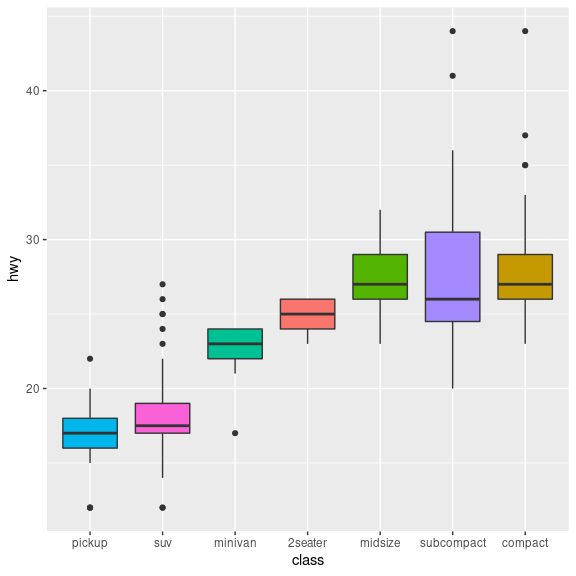
\includegraphics[width=3.125in,height=\textheight]{images/rmarkdown/000002.png}
\caption{자동차 모델에 따른 고속도로 연비 분포}
\end{figure}

\begin{enumerate}
\def\labelenumi{\arabic{enumi}.}
\tightlist
\item
  첫 번째
\item
  두 번째
\item
  세 번째
\end{enumerate}

\begin{itemize}
\tightlist
\item
  아이템 1
\item
  아이템 2
\item
  아이템 3

  \begin{itemize}
  \tightlist
  \item
    아이템 3-1
  \item
    아이템 3-2
  \end{itemize}
\end{itemize}

소스코드 그대로 표현하기 위해서는 \texttt{\textasciitilde{}\textasciitilde{}\textasciitilde{}} 를 사용합니다.

\begin{verbatim}
<div>
  소스코드 
</div>
\end{verbatim}

\hypertarget{yaml-uxd5e4uxb354}{%
\section{YAML 헤더}\label{yaml-uxd5e4uxb354}}

R markdown 파일에서 YAML의 가장 중요한 기능은 output 포멧을 지정하는 것이며 title, author, date, 등을 설정할수도 있습니다.

\begin{verbatim}
---
layout: page
title: "R프로그래밍"
subtitle: "R markdown 활용법"
output:
  html_document:
    css: style.css
    includes:
      in_header: header.html
      after_body: footer.html
    theme: default
    toc: yes
    toc_float: true
    highlight: tango
    code_folding: show
    number_sections: TRUE
mainfont: NanumGothic
---
\end{verbatim}

\hypertarget{output-format}{%
\section{Output format}\label{output-format}}

주요 문서 포멧으로 다음과 같은 몇 가지가 있습니다. 상세한 내용은 \href{https://rmarkdown.rstudio.com/lesson-9.html}{Rmarkdown output format}을 참고하시기 바랍니다.

\begin{itemize}
\tightlist
\item
  html\_document - HTML document w/ Bootstrap CSS
\item
  pdf\_document - PDF document (via LaTeX template)
\item
  word\_document - Microsoft Word document (docx)
\item
  ioslides\_presentation - HTML presentation with ioslides
\item
  beamer\_presentation - PDF presentation with LaTeX Beamer
\item
  powerpoint\_presentation: PowerPoint presentation
\end{itemize}

\begin{center}\rule{0.5\linewidth}{0.5pt}\end{center}

이 저작물은 크리에이티브 커먼즈 저작자표시-비영리-변경금지 4.0 국제 라이선스에 따라 이용할 수 있습니다.

\hypertarget{r-programming}{%
\chapter{R programming}\label{r-programming}}

\hypertarget{console-calculator}{%
\section{Console calculator}\label{console-calculator}}

콘솔에서 바로 계산을 수행할 수 있습니다. 참고로 이전에 수행한 명령은 콘솔에 커서가 있는 상태에서 위 아래 화살표를 누르면 볼 수 있고 엔터를 눌러 재사용 할 수 있습니다. \texttt{;}을 사용하면 두 개의 명령을 동시에 수행할 수 있습니다.

\[ 2 + 2 \]
\[ ((2 - 1)^2 + (1 - 3)^2)^{1/2} \]

\begin{Shaded}
\begin{Highlighting}[]
\DecValTok{2} \SpecialCharTok{+} \DecValTok{2}
\NormalTok{((}\DecValTok{2}\NormalTok{ – }\DecValTok{1}\NormalTok{)}\SpecialCharTok{\^{}}\DecValTok{2} \SpecialCharTok{+}\NormalTok{ (}\DecValTok{1}\NormalTok{ – }\DecValTok{3}\NormalTok{)}\SpecialCharTok{\^{}}\DecValTok{2}\NormalTok{ )}\SpecialCharTok{\^{}}\NormalTok{(}\DecValTok{1}\SpecialCharTok{/}\DecValTok{2}\NormalTok{)}
\DecValTok{2} \SpecialCharTok{+} \DecValTok{2}\NormalTok{; }\DecValTok{2} \SpecialCharTok{{-}} \DecValTok{2}
\end{Highlighting}
\end{Shaded}

\hypertarget{exercise-1}{%
\subsection*{Exercise}\label{exercise-1}}
\addcontentsline{toc}{subsection}{Exercise}

다음 공식들을 계산하는 R 코드를 작성하시오

\[ \sqrt{(4+3)(2+1)} \]

\[ 2^3 + 3^2 \]

\[ \frac{0.25 - 0.2}{\sqrt{0.2 (1-0.2)/100}}\]

\hypertarget{what-is-a-programming-language}{%
\section{What is a programming language}\label{what-is-a-programming-language}}

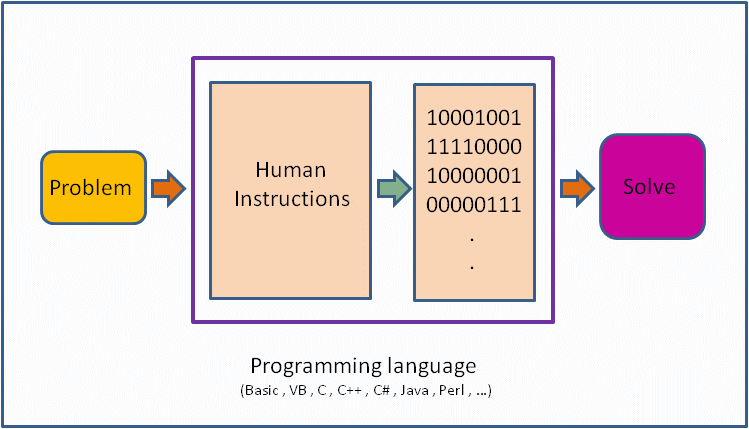
\includegraphics[width=6.25in,height=\textheight]{images/01/24.PNG}
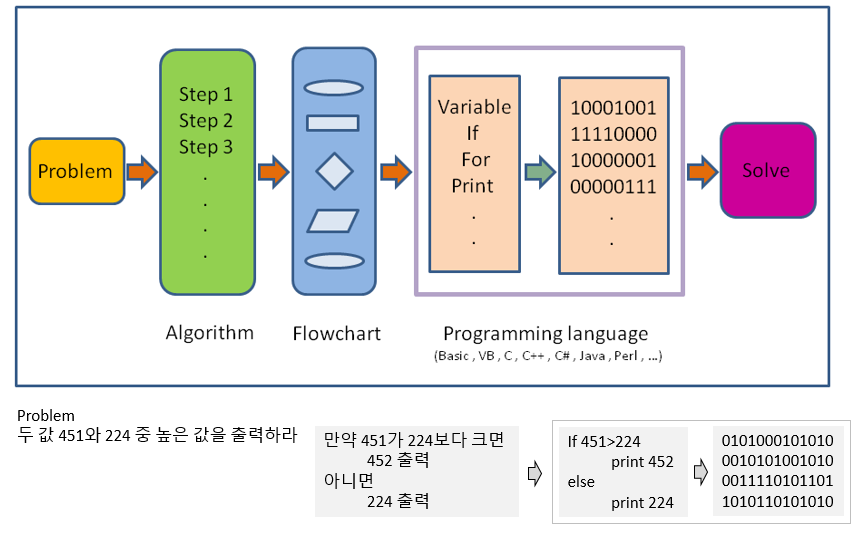
\includegraphics[width=6.45833in,height=\textheight]{images/01/25.PNG}

R은 programming language로서 다른 프로그래밍 언어와 같이 몇 가지 공통적 개념을 가집니다 (\texttt{변수}, \texttt{자료형}, \texttt{함수}, \texttt{조건문}, \texttt{반복문})

\hypertarget{terminology}{%
\subsection{Terminology}\label{terminology}}

\begin{itemize}
\tightlist
\item
  Session: R 언어 실행 환경
\item
  Console: 명령어 입력하는 창
\item
  Code: R 프로그래밍 변수/제어문 모음
\item
  Object: 변수, 함수 등 프로그래밍에서 사용되는 모든 객체 (Data structure)

  \begin{itemize}
  \tightlist
  \item
    array: 1D, 2D, 3D, \ldots{} 형태 값들의 모임
  \item
    vector: 1차원 형태 값들의 모임 combine function \texttt{c()} EX: c(6, 11, 13, 31, 90, 92)
  \item
    matrix: 2차원 형태 값들의 모임 (같은 타입 값으로 구성)
  \item
    data frame: 2차원 형태 값들의 모임 (다른 타입 값 구성 가능)
  \item
    list: vector, matrix, data.frame 및 list 등 다양한 객체를 원소로 가집
  \end{itemize}
\item
  function: 특정 기능 수행, {[}함수이름, 입력값 (arguments), 출력값 (return){]} 으로 구성
\item
  Data (value): 값 - 자료형 (Data type)

  \begin{itemize}
  \tightlist
  \item
    Integers
  \item
    doubles/numerics
  \item
    logicals
  \item
    characters
  \item
    factor: 범주형
  \end{itemize}
\item
  Conditionals (조건, 제어):

  \begin{itemize}
  \tightlist
  \item
    \texttt{if}, \texttt{==}, \texttt{\&} (AND), \texttt{\textbar{}} (OR) Ex: \texttt{(2\ +\ 1\ ==\ 3)\ \&\ (2\ +\ 1\ ==\ 4)}
  \item
    \texttt{for}, \texttt{while}: 반복 수
  \end{itemize}
\end{itemize}

\hypertarget{data-and-variables}{%
\section{Data and variables}\label{data-and-variables}}

\hypertarget{data}{%
\subsection{Data}\label{data}}

일반적으로 데이터의 의미는 사실을 나타내는 수치입니다.

\begin{itemize}
\tightlist
\item
  맥도너 정보경제학 (1963)

  \begin{itemize}
  \tightlist
  \item
    지혜 (wisdom) : 패턴화된 지식
  \item
    지식 (knowledge) : 가치있는 정보
  \item
    정보 (information) : 의미있는 데이터
  \item
    데이터 (data) : 단순한 사실의 나열
  \end{itemize}
\end{itemize}

\begin{Shaded}
\begin{Highlighting}[]
\FunctionTok{library}\NormalTok{(UsingR)}
\NormalTok{exec.pay}
\NormalTok{?exec.pay}
\end{Highlighting}
\end{Shaded}

데이터는 속성에 따라서 다음과 같이 분류할 수 있습니다.

\begin{itemize}
\tightlist
\item
  범주형 - 질적 데이터, 숫자로 나타낼 수 있으나 의미 없음

  \begin{itemize}
  \tightlist
  \item
    명목형 (Nominal) - 사람 이름
  \item
    순서형 (Ordinal) -- 달리기 도착 순서
  \end{itemize}
\item
  수치형 - 숫자로 나타내며 데이터 속성을 그대로 지님님

  \begin{itemize}
  \tightlist
  \item
    구간형 (Interval) -- 선수1, 선수2 종점통과 시간
  \item
    비율형 (Ratio) -- 출발시간 기준 종점 통과 시간
  \end{itemize}
\end{itemize}

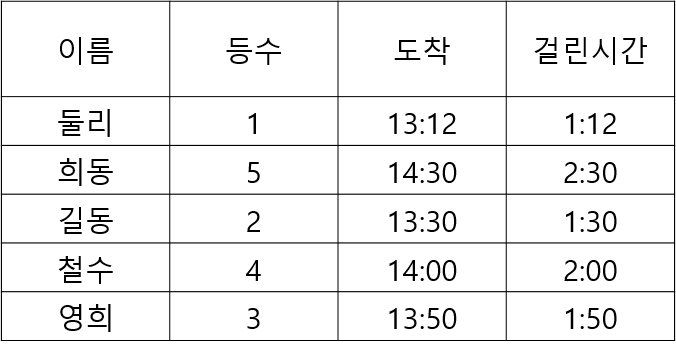
\includegraphics[width=4.16667in,height=\textheight]{images/02/01.png}

\begin{itemize}
\tightlist
\item
  Data type in R

  \begin{itemize}
  \tightlist
  \item
    Numeric (수치형)

    \begin{itemize}
    \tightlist
    \item
      Discrete (이산형) data - 카운트, 횟수
    \item
      Continuous (연속형) data - 키, 몸무게, Cannot be shared
    \item
      Date and time
    \end{itemize}
  \item
    Factors (범주형)

    \begin{itemize}
    \tightlist
    \item
      Categories to group the data
    \item
      Character data - Identifiers (범주형)
    \end{itemize}
  \end{itemize}
\end{itemize}

\hypertarget{variables}{%
\subsection{Variables}\label{variables}}

변수는 데이터를 저장하는 공간으로 이해할 수 있습니다.

\begin{itemize}
\tightlist
\item
  Assignment operator ( \texttt{\textless{}-} OR \texttt{=} )

  \begin{itemize}
  \tightlist
  \item
    Valid object name \texttt{\textless{}-} value
  \item
    단축키: \texttt{Alt\ +\ -} (the minus sign)
  \end{itemize}
\item
  내장 변수 Built-in variables
\end{itemize}

\begin{Shaded}
\begin{Highlighting}[]
\NormalTok{x }\OtherTok{\textless{}{-}} \DecValTok{2}
\NormalTok{y }\OtherTok{\textless{}{-}}\NormalTok{ x}\SpecialCharTok{\^{}}\DecValTok{2}\NormalTok{ – }\DecValTok{2}\SpecialCharTok{*}\NormalTok{x }\SpecialCharTok{+} \DecValTok{1}
\NormalTok{y}
\NormalTok{x }\OtherTok{\textless{}{-}} \StringTok{"two"}  
\NormalTok{some\_data }\OtherTok{\textless{}{-}} \FloatTok{9.8}
\NormalTok{pi}
\end{Highlighting}
\end{Shaded}

\begin{itemize}
\tightlist
\item
  변수이름 작명법

  \begin{itemize}
  \tightlist
  \item
    Characters (letters), numbers, ``\_'', ``.''
  \item
    A and a are different symbols
  \item
    Names are effectively unlimited in length
  \end{itemize}
\end{itemize}

\begin{Shaded}
\begin{Highlighting}[]
\NormalTok{i\_use\_snake\_case }\OtherTok{\textless{}{-}} \DecValTok{1}
\NormalTok{otherPeopleUseCamelCase }\OtherTok{\textless{}{-}} \DecValTok{2}
\NormalTok{some.people.use.periods }\OtherTok{\textless{}{-}} \DecValTok{3}
\NormalTok{And\_aFew.People\_RENOUNCEconvention }\OtherTok{\textless{}{-}} \DecValTok{4}
\end{Highlighting}
\end{Shaded}

\hypertarget{object-data-structure}{%
\section{Object (Data structure)}\label{object-data-structure}}

변수, 함수 등 프로그래밍에서 사용되는 모든 개체를 말합니다.

\hypertarget{vector}{%
\subsection{vector}\label{vector}}

\texttt{vector}는 R의 기본 데이터 구조입니다. numeric vector, logical vector, character vector 등 저장되는 값의 타입에 따라 크게 세가지로 나눌 수 있습니다. \texttt{class()} 함수를 이용해서 값의 타입을 알아낼 수 있습니다. Combine function인 \texttt{c()}를 활용하여 만들며 값을 순차적으로 붙여갈 수 있습니다. 다음과 같은 Univariate (단변량, Single variable)을 표현할 때 사용됩니다.

\[ x_1, x_2, ..., x_n \]

\begin{Shaded}
\begin{Highlighting}[]
\NormalTok{x }\OtherTok{\textless{}{-}} \FunctionTok{c}\NormalTok{(}\FloatTok{10.4}\NormalTok{, }\FloatTok{5.6}\NormalTok{, }\FloatTok{3.1}\NormalTok{, }\FloatTok{6.4}\NormalTok{, }\FloatTok{21.7}\NormalTok{) }
\FunctionTok{class}\NormalTok{(x)}
\NormalTok{y }\OtherTok{\textless{}{-}} \FunctionTok{c}\NormalTok{(}\StringTok{"X1"}\NormalTok{, }\StringTok{"Y2"}\NormalTok{,  }\StringTok{"X3"}\NormalTok{,  }\StringTok{"Y4"}\NormalTok{)}
\FunctionTok{class}\NormalTok{(y)}
\NormalTok{z }\OtherTok{\textless{}{-}} \FunctionTok{c}\NormalTok{(T, F, F, T)}
\FunctionTok{class}\NormalTok{(z)}
\end{Highlighting}
\end{Shaded}

\hypertarget{numeric}{%
\subsubsection{numeric}\label{numeric}}

numeric 형식의 벡터는 다음과 같은 다양한 편의 함수들을 사용해서 만들수 있습니다.

\begin{Shaded}
\begin{Highlighting}[]
\DecValTok{1}\SpecialCharTok{:}\DecValTok{5}
\FunctionTok{seq}\NormalTok{(}\DecValTok{1}\NormalTok{,}\DecValTok{5}\NormalTok{, }\AttributeTok{by=}\DecValTok{1}\NormalTok{)}
\FunctionTok{seq}\NormalTok{(}\DecValTok{0}\NormalTok{, }\DecValTok{100}\NormalTok{, }\AttributeTok{by=}\DecValTok{10}\NormalTok{)}
\FunctionTok{seq}\NormalTok{(}\DecValTok{0}\NormalTok{, }\DecValTok{100}\NormalTok{, }\AttributeTok{length.out=}\DecValTok{11}\NormalTok{)}
\NormalTok{?seq}

\FunctionTok{rep}\NormalTok{(}\DecValTok{5}\NormalTok{, }\AttributeTok{times=}\DecValTok{10}\NormalTok{)}
\FunctionTok{rep}\NormalTok{(}\DecValTok{1}\SpecialCharTok{:}\DecValTok{3}\NormalTok{, }\AttributeTok{times=}\DecValTok{4}\NormalTok{)}
\FunctionTok{rep}\NormalTok{(}\DecValTok{1}\SpecialCharTok{:}\DecValTok{3}\NormalTok{, }\AttributeTok{each=}\DecValTok{3}\NormalTok{)}
\end{Highlighting}
\end{Shaded}

\hypertarget{exercise-2}{%
\subsubsection*{Exercise}\label{exercise-2}}
\addcontentsline{toc}{subsubsection}{Exercise}

odds라는 이름의 변수에 1부터 100까지의 홀수만을 저장하시오 (\texttt{seq()} 함수 사용)

\hypertarget{logical}{%
\subsubsection{logical}\label{logical}}

Logical 벡터는 \texttt{True} 또는 \texttt{False}를 원소로 갖는 벡터 입니다. 앞글자가 대분자로 시작하는 것을 기억하시고 \texttt{T} 또는 \texttt{F}와 같이 한 문자로 표현할 수도 있습니다. 특정 조건에 대한 판단 결과를 반환할 경우에도 논리값을 사용합니다. 이 경우 조건을 판단 후 인덱싱 방법으로 해당 값들을 뽑아내기도 합니다.

\begin{Shaded}
\begin{Highlighting}[]
\FunctionTok{is.na}\NormalTok{(}\DecValTok{1}\NormalTok{)}
\FunctionTok{is.numeric}\NormalTok{(}\DecValTok{1}\NormalTok{)}
\FunctionTok{is.logical}\NormalTok{(}\ConstantTok{TRUE}\NormalTok{)}

\NormalTok{x }\OtherTok{\textless{}{-}} \DecValTok{1}\SpecialCharTok{:}\DecValTok{20}
\NormalTok{x }\SpecialCharTok{\textgreater{}} \DecValTok{13}
\NormalTok{temp }\OtherTok{\textless{}{-}}\NormalTok{ x }\SpecialCharTok{\textgreater{}} \DecValTok{13}
\FunctionTok{class}\NormalTok{(temp)}

\NormalTok{ages }\OtherTok{\textless{}{-}} \FunctionTok{c}\NormalTok{(}\DecValTok{66}\NormalTok{, }\DecValTok{57}\NormalTok{, }\DecValTok{60}\NormalTok{, }\DecValTok{41}\NormalTok{,  }\DecValTok{6}\NormalTok{, }\DecValTok{85}\NormalTok{, }\DecValTok{48}\NormalTok{, }\DecValTok{34}\NormalTok{, }\DecValTok{61}\NormalTok{, }\DecValTok{12}\NormalTok{)}
\NormalTok{ages }\SpecialCharTok{\textless{}} \DecValTok{30}
\FunctionTok{which}\NormalTok{(ages }\SpecialCharTok{\textless{}} \DecValTok{30}\NormalTok{)}
\NormalTok{i }\OtherTok{\textless{}{-}} \FunctionTok{which}\NormalTok{(ages }\SpecialCharTok{\textless{}} \DecValTok{30}\NormalTok{)}
\NormalTok{ages[i]}
\FunctionTok{any}\NormalTok{(ages }\SpecialCharTok{\textless{}} \DecValTok{30}\NormalTok{)}
\FunctionTok{all}\NormalTok{(ages }\SpecialCharTok{\textless{}} \DecValTok{30}\NormalTok{)}
\end{Highlighting}
\end{Shaded}

\hypertarget{exercise-3}{%
\subsubsection*{Exercise}\label{exercise-3}}
\addcontentsline{toc}{subsubsection}{Exercise}

1부터 100까지의 수를 n이라는 이름의 변수에 저장하고 이 중 짝수만을 뽑아내서 출력하시오 (\texttt{which()}함수 사용)

\hypertarget{character}{%
\subsubsection{character}\label{character}}

Character(문자형) 벡터의 경우 문자열을 다루는데 자주 쓰이는 \texttt{paste()} 함수의 사용법을 알아두면 편리합니다. \texttt{paste()} 함수는 서로 다른 문자열을 붙이는데 주로 사용됩니다. 참고로 문자열을 나누는 함수는 \texttt{strsplit()} 입니다. \texttt{paste()}에서 붙이는 문자 사이에 들어가는 문자를 지정하는 파라메터는 \texttt{sep} 이고 \texttt{strsplit()}함수에서 자르는 기준이 되는 문자는\texttt{split} 파라메터로 지정해 줍니다 (\texttt{?split} 또는 \texttt{?paste} 확인).

\begin{Shaded}
\begin{Highlighting}[]
\FunctionTok{paste}\NormalTok{(}\StringTok{"X"}\NormalTok{, }\StringTok{"Y"}\NormalTok{, }\StringTok{"Z"}\NormalTok{, }\AttributeTok{sep=}\StringTok{"\_"}\NormalTok{)}
\FunctionTok{paste}\NormalTok{(}\FunctionTok{c}\NormalTok{(}\StringTok{"Four"}\NormalTok{,}\StringTok{"The"}\NormalTok{), }\FunctionTok{c}\NormalTok{(}\StringTok{"Score"}\NormalTok{,}\StringTok{"quick"}\NormalTok{), }\FunctionTok{c}\NormalTok{(}\StringTok{"and"}\NormalTok{,}\StringTok{"fox"}\NormalTok{), }\AttributeTok{sep=}\StringTok{"\_"}\NormalTok{)}
\FunctionTok{paste}\NormalTok{(}\StringTok{"X"}\NormalTok{, }\DecValTok{1}\SpecialCharTok{:}\DecValTok{5}\NormalTok{, }\AttributeTok{sep=}\StringTok{""}\NormalTok{)}
\FunctionTok{paste}\NormalTok{(}\FunctionTok{c}\NormalTok{(}\StringTok{"X"}\NormalTok{,}\StringTok{"Y"}\NormalTok{), }\DecValTok{1}\SpecialCharTok{:}\DecValTok{10}\NormalTok{, }\AttributeTok{sep=}\StringTok{""}\NormalTok{)}

\NormalTok{x }\OtherTok{\textless{}{-}} \FunctionTok{c}\NormalTok{(}\StringTok{"X1"}\NormalTok{, }\StringTok{"Y2"}\NormalTok{, }\StringTok{"X3"}\NormalTok{, }\StringTok{"Y4"}\NormalTok{, }\StringTok{"X5"}\NormalTok{)}
\FunctionTok{paste}\NormalTok{(x[}\DecValTok{1}\NormalTok{], x[}\DecValTok{2}\NormalTok{])}
\FunctionTok{paste}\NormalTok{(x[}\DecValTok{1}\NormalTok{], x[}\DecValTok{2}\NormalTok{], }\AttributeTok{sep=}\StringTok{""}\NormalTok{)}
\FunctionTok{paste}\NormalTok{(x, }\AttributeTok{collapse=}\StringTok{"\_"}\NormalTok{)}

\FunctionTok{strsplit}\NormalTok{(}\StringTok{"XYZ"}\NormalTok{, }\AttributeTok{split=}\StringTok{""}\NormalTok{)}
\end{Highlighting}
\end{Shaded}

\hypertarget{exercise-4}{%
\subsubsection*{Exercise}\label{exercise-4}}
\addcontentsline{toc}{subsubsection}{Exercise}

\texttt{m}이라는 변수에 ``Capital of South Korea is Seoul'' 문자열을 저장하고 ``Capital of South Korea''를 따로 뽑아내 \texttt{m2}에 저장하시오 (\texttt{substr()} 사용)

\hypertarget{factor}{%
\subsubsection{factor}\label{factor}}

Factor형은 범주형데이터를 저장하기 위한 object 이며 R 언어에서 특별히 만들어져 사용되고 있습니다. \texttt{factor()} 함수를 이용해 생성하며 생성된 객체는 다음과 같이 \texttt{level}이라는 범주를 나타내는 특성값을 가지고 있습니다.

\begin{Shaded}
\begin{Highlighting}[]
\NormalTok{x }\OtherTok{\textless{}{-}} \FunctionTok{c}\NormalTok{(}\StringTok{"Red"}\NormalTok{, }\StringTok{"Blue"}\NormalTok{, }\StringTok{"Yellow"}\NormalTok{, }\StringTok{"Green"}\NormalTok{, }\StringTok{"Blue"}\NormalTok{, }\StringTok{"Green"}\NormalTok{)}
\NormalTok{y }\OtherTok{\textless{}{-}} \FunctionTok{factor}\NormalTok{(x)}
\NormalTok{y}
\end{Highlighting}
\end{Shaded}

새로운 범주의 데이터를 추가할 경우 다음과 같이 해당되는 level을 먼저 추가하고 값을 저장해야 합니다.

\begin{Shaded}
\begin{Highlighting}[]
\FunctionTok{levels}\NormalTok{(y)}
\NormalTok{y[}\DecValTok{1}\NormalTok{] }\OtherTok{\textless{}{-}} \StringTok{"Gold"}
\NormalTok{y}

\FunctionTok{levels}\NormalTok{(y) }\OtherTok{\textless{}{-}} \FunctionTok{c}\NormalTok{(}\FunctionTok{levels}\NormalTok{(y), }\StringTok{"Gold"}\NormalTok{)}
\FunctionTok{levels}\NormalTok{(y)}
\NormalTok{y}
\NormalTok{y[}\DecValTok{1}\NormalTok{] }\OtherTok{\textless{}{-}} \StringTok{"Gold"}
\NormalTok{y}
\end{Highlighting}
\end{Shaded}

\texttt{factor}는 기본적으로 \texttt{level}에 표시된 순서가 위치 (정렬) 순서입니다. 이를 바꾸기 위해서는 다음과 같이 \texttt{levels} 함수를 이용해서 순서를 바꿀 수 있습니다.

\begin{Shaded}
\begin{Highlighting}[]
\CommentTok{\#library(UsingR)}
\FunctionTok{str}\NormalTok{(Cars93)}
\NormalTok{x }\OtherTok{\textless{}{-}}\NormalTok{ Cars93}\SpecialCharTok{$}\NormalTok{Origin}
\FunctionTok{plot}\NormalTok{(x)}
\FunctionTok{levels}\NormalTok{(x) }\OtherTok{\textless{}{-}} \FunctionTok{c}\NormalTok{(}\StringTok{"non{-}USA"}\NormalTok{, }\StringTok{"USA"}\NormalTok{)}
\FunctionTok{levels}\NormalTok{(x)}
\FunctionTok{plot}\NormalTok{(x)}
\end{Highlighting}
\end{Shaded}

\hypertarget{attribute}{%
\subsubsection{Attribute}\label{attribute}}

vector 들은 다음과 같은 builtin 함수들을 사용해서 해당 변수의 attribute를 알아낼 수 있습니다. attribute에는 원소 이름, 타입, 길이 등 vector형 변수가 가질 수 있는 특성을 말합니다.

\begin{Shaded}
\begin{Highlighting}[]
\FunctionTok{head}\NormalTok{(precip)}
\FunctionTok{class}\NormalTok{(precip)}
\FunctionTok{length}\NormalTok{(precip)}
\FunctionTok{names}\NormalTok{(precip)}

\NormalTok{test\_scores }\OtherTok{\textless{}{-}} \FunctionTok{c}\NormalTok{(}\DecValTok{100}\NormalTok{, }\DecValTok{90}\NormalTok{, }\DecValTok{80}\NormalTok{)}
\FunctionTok{names}\NormalTok{(test\_scores) }\OtherTok{\textless{}{-}} \FunctionTok{c}\NormalTok{(}\StringTok{"Alice"}\NormalTok{, }\StringTok{"Bob"}\NormalTok{, }\StringTok{"Shirley"}\NormalTok{)}
\NormalTok{test\_scores}
\end{Highlighting}
\end{Shaded}

\hypertarget{indexing}{%
\subsubsection{indexing}\label{indexing}}

인덱싱은 vector 데이터의 일부 데이터를 참조할 때 사용하는 방법입니다.

\begin{Shaded}
\begin{Highlighting}[]
\NormalTok{x[}\DecValTok{1}\NormalTok{]}
\NormalTok{x[}\DecValTok{1}\SpecialCharTok{:}\DecValTok{3}\NormalTok{]}
\NormalTok{i }\OtherTok{\textless{}{-}} \DecValTok{1}\SpecialCharTok{:}\DecValTok{3}
\NormalTok{x[i]}
\NormalTok{x[}\FunctionTok{c}\NormalTok{(}\DecValTok{1}\NormalTok{,}\DecValTok{2}\NormalTok{,}\DecValTok{4}\NormalTok{)]}
\NormalTok{y[}\DecValTok{3}\NormalTok{]}

\FunctionTok{head}\NormalTok{(precip)}
\NormalTok{precip[}\DecValTok{1}\NormalTok{]}
\NormalTok{precip[}\DecValTok{2}\SpecialCharTok{:}\DecValTok{10}\NormalTok{]}
\NormalTok{precip[}\FunctionTok{c}\NormalTok{(}\DecValTok{1}\NormalTok{,}\DecValTok{3}\NormalTok{,}\DecValTok{5}\NormalTok{)]}
\NormalTok{precip[}\SpecialCharTok{{-}}\DecValTok{1}\NormalTok{]}
\NormalTok{precip[}\StringTok{"Seattle Tacoma"}\NormalTok{]}
\NormalTok{precip[}\FunctionTok{c}\NormalTok{(}\StringTok{"Seattle Tacoma"}\NormalTok{, }\StringTok{"Portland"}\NormalTok{)]}
\NormalTok{precip[}\DecValTok{2}\NormalTok{] }\OtherTok{\textless{}{-}} \DecValTok{10}
\end{Highlighting}
\end{Shaded}

\hypertarget{missing-values}{%
\subsubsection{Missing values}\label{missing-values}}

특정 값이 ``Not available'' 이거나 ``Missing value'' 일 경우 벡터의 해당 원소 자리에 데이터의 이상을 알리기 위해 \texttt{NA}를 사용합니다. 따라서 일반적인 연산에서 \texttt{NA}가 포함되어 있는 경우 데이터의 불완전성을 알리기 위해 연산의 결과는 \texttt{NA}가 됩니다. \texttt{is.na()} 함수는 해당 변수에 \texttt{NA} 값이 있는지를 검사해주는 함수이며 R에는 이 외에도 다음과 같은 특수 값들이 사용되고 있습니다.

\begin{itemize}
\tightlist
\item
  NA: Not available, The value is missing
\item
  NULL: a reserved value
\item
  NaN: Not a number (0/0)
\item
  Inf: (1/0)
\end{itemize}

\begin{Shaded}
\begin{Highlighting}[]
\NormalTok{hip\_cost }\OtherTok{\textless{}{-}} \FunctionTok{c}\NormalTok{(}\DecValTok{10500}\NormalTok{, }\DecValTok{45000}\NormalTok{, }\DecValTok{74100}\NormalTok{, }\ConstantTok{NA}\NormalTok{, }\DecValTok{83500}\NormalTok{)}
\FunctionTok{sum}\NormalTok{(hip\_cost)}
\FunctionTok{sum}\NormalTok{(hip\_cost, }\AttributeTok{na.rm=}\ConstantTok{TRUE}\NormalTok{)}
\NormalTok{?sum}
\end{Highlighting}
\end{Shaded}

\hypertarget{useful-functions}{%
\subsubsection{Useful functions}\label{useful-functions}}

다음은 벡터형 변수와 같이 쓰이는 유용한 함수들입니다.

\begin{Shaded}
\begin{Highlighting}[]
\NormalTok{z }\OtherTok{\textless{}{-}} \FunctionTok{sample}\NormalTok{(}\DecValTok{1}\SpecialCharTok{:}\DecValTok{10}\NormalTok{, }\DecValTok{100}\NormalTok{, T)}
\FunctionTok{head}\NormalTok{(z)}
\FunctionTok{sort}\NormalTok{(z)}
\FunctionTok{order}\NormalTok{(z)}
\FunctionTok{table}\NormalTok{(z)}
\NormalTok{p }\OtherTok{\textless{}{-}}\NormalTok{ z}\SpecialCharTok{/}\FunctionTok{sum}\NormalTok{(z)}
\FunctionTok{round}\NormalTok{(p, }\AttributeTok{digits=}\DecValTok{1}\NormalTok{)}
\NormalTok{digits }\OtherTok{\textless{}{-}} \FunctionTok{as.character}\NormalTok{(z)}
\NormalTok{n }\OtherTok{\textless{}{-}} \FunctionTok{as.numeric}\NormalTok{(digits)}
\NormalTok{d }\OtherTok{\textless{}{-}} \FunctionTok{as.integer}\NormalTok{(digits)}
\end{Highlighting}
\end{Shaded}

\hypertarget{matrix}{%
\subsection{matrix}\label{matrix}}

매트릭스는 2차원 행렬로 같은 형식의 데이터 값 (numberic, character, logical) 으로만 채워진 행렬을 말합니다. 메트릭스를 만드는 방법은 아래와 같으며 \texttt{nrow} 와 \texttt{ncol} 파라메터에 행과 열의 수를 넣고 각 셀에 들어갈 값은 가장 앞에 위치한 data 파라메터에 넣어 줍니다 (\texttt{?matrix}로 파라메터 이름 확인). 메트릭스 인덱싱은 메트릭스 안의 값을 저장하거나 참조할때 (빼올때) 사용하는 방법입니다. 메트릭스 변수이름 바로 뒤에 대괄호를 이용해서 제어를 하며 대괄호 안에 콤마로 구분된 앞쪽은 row, 뒷쪽은 column 인덱스를 나타냅니다.

\begin{Shaded}
\begin{Highlighting}[]
\NormalTok{mymat }\OtherTok{\textless{}{-}} \FunctionTok{matrix}\NormalTok{(}\DecValTok{0}\NormalTok{, }\AttributeTok{nrow=}\DecValTok{100}\NormalTok{, }\AttributeTok{ncol=}\DecValTok{3}\NormalTok{) }\CommentTok{\# 1}
\NormalTok{mymat[,}\DecValTok{1}\NormalTok{] }\OtherTok{\textless{}{-}} \DecValTok{1}\SpecialCharTok{:}\DecValTok{100} \CommentTok{\# 2}
\NormalTok{mymat[,}\DecValTok{2}\NormalTok{] }\OtherTok{\textless{}{-}} \FunctionTok{seq}\NormalTok{(}\DecValTok{1}\NormalTok{,}\DecValTok{200}\NormalTok{,}\DecValTok{2}\NormalTok{) }\CommentTok{\# 3}
\NormalTok{mymat[,}\DecValTok{3}\NormalTok{] }\OtherTok{\textless{}{-}} \FunctionTok{seq}\NormalTok{(}\DecValTok{2}\NormalTok{,}\DecValTok{200}\NormalTok{,}\DecValTok{2}\NormalTok{) }\CommentTok{\# 4}
\end{Highlighting}
\end{Shaded}

매트릭스의 row나 column에 이름이 주어져 있을 경우 이름을 따옴표(``)로 묶은 후 참조가 가능합니다. row나 column의 이름은 \texttt{rownames()} 또는 \texttt{colnames()}로 생성하거나 변경할 수 있습니다. row나 column의 개수는 \texttt{nrow()} 또는 \texttt{ncol()} 함수를 사용합니다.

\begin{Shaded}
\begin{Highlighting}[]
\FunctionTok{colnames}\NormalTok{(mymat)}
\FunctionTok{colnames}\NormalTok{(mymat) }\OtherTok{\textless{}{-}} \FunctionTok{c}\NormalTok{(}\StringTok{"A"}\NormalTok{, }\StringTok{"B"}\NormalTok{, }\StringTok{"C"}\NormalTok{)}
\FunctionTok{colnames}\NormalTok{(mymat)}
\FunctionTok{colnames}\NormalTok{(mymat)[}\DecValTok{2}\NormalTok{] }\OtherTok{\textless{}{-}} \StringTok{"D"}
\FunctionTok{colnames}\NormalTok{(mymat)}
\FunctionTok{rownames}\NormalTok{(mymat) }\OtherTok{\textless{}{-}} \FunctionTok{paste}\NormalTok{(}\StringTok{"No"}\NormalTok{, }\DecValTok{1}\SpecialCharTok{:}\FunctionTok{nrow}\NormalTok{(mymat), }\AttributeTok{sep=}\StringTok{""}\NormalTok{)}
\FunctionTok{rownames}\NormalTok{(mymat)}
\end{Highlighting}
\end{Shaded}

여러 row나 column을 참조할 경우 아래와 같이 combine 함수를 사용하여 묶어줘야 하며 스칼라값을 (임의의 숫자 하나) 더하거나 뺄 경우 vector / matrix 연산을 기본으로 수행합니다.

\begin{Shaded}
\begin{Highlighting}[]
\NormalTok{mymat[}\FunctionTok{c}\NormalTok{(}\DecValTok{2}\NormalTok{,}\DecValTok{3}\NormalTok{,}\DecValTok{4}\NormalTok{,}\DecValTok{5}\NormalTok{),}\DecValTok{2}\NormalTok{] }\CommentTok{\# 5}
\NormalTok{mymat}\DecValTok{{-}1} \CommentTok{\# 6}
\NormalTok{mysub }\OtherTok{\textless{}{-}}\NormalTok{ mymat[,}\DecValTok{2}\NormalTok{] }\SpecialCharTok{{-}}\NormalTok{ mymat[,}\DecValTok{1}\NormalTok{] }\CommentTok{\#7}
\FunctionTok{sum}\NormalTok{(mysub) }\CommentTok{\#8}
\FunctionTok{sum}\NormalTok{(mysub}\SpecialCharTok{\^{}}\DecValTok{2}\NormalTok{) }\CommentTok{\#8}
\end{Highlighting}
\end{Shaded}

\hypertarget{exercise-5}{%
\subsubsection*{Exercise}\label{exercise-5}}
\addcontentsline{toc}{subsubsection}{Exercise}

\begin{itemize}
\tightlist
\item
  score 라는 변수에 1부터 100까지 중 랜덤하게 선택된 20개의 수로 10 x 2 matrix를 만드시오 (\texttt{sample()} 사용)
\item
  score의 row 이름을 문자형으로 Name1, Name2, \ldots, Name10으로 지정하시오 (\texttt{paste()} 사용)
\item
  score의 column 이름을 문자형으로 math와 eng로 지정하시오
\item
  이 matrix의 첫번째 컬럼과 두 번째 컬럼의 수를 각각 더한 후 \texttt{total\_score}라는 변수에 저장하시오
\item
  \texttt{total\_score}의의 오름차순 순서를 나타내는 인덱스 (\texttt{order()}함수 사용)를 \texttt{o}라는 변수에 저장하시오
\item
  score를 \texttt{o}순서로 재배치하고 score\_ordered 변수에 저장하시오
\end{itemize}

\hypertarget{data.frame}{%
\subsection{data.frame}\label{data.frame}}

데이터프레임은 형태는 매트릭스와 같으나 컬럼 하나가 하나의 변수로서 각 변수들이 다른 모드의 값을 저장할 수 있다는 차이가 있습니다. \texttt{\$} 기호를 이용하여 각 구성 변수를 참조할 수 있습니다. 컬럼 한 줄이 하나의 변수 이므로 새로운 변수도 컬럼 형태로 붙여 넣을 수 있습니다. 즉, 각 row는 샘플을 나타내고 각 column은 변수를 나타내며 각 변수들이 갖는 샘플의 개수 (row의 길이, vector 의 길이)는 같아야 합니다. R 기반의 데이터 분석에서는 가장 선호되는 데이터 타입이라고 볼 수 있습니다.

\begin{Shaded}
\begin{Highlighting}[]
\DocumentationTok{\#\# data.frame}
\NormalTok{ids }\OtherTok{\textless{}{-}} \DecValTok{1}\SpecialCharTok{:}\DecValTok{10}
\NormalTok{ids}
\NormalTok{idnames }\OtherTok{\textless{}{-}} \FunctionTok{paste}\NormalTok{(}\StringTok{"Name"}\NormalTok{, ids, }\AttributeTok{sep=}\StringTok{""}\NormalTok{)}
\NormalTok{idnames}
\NormalTok{students }\OtherTok{\textless{}{-}} \FunctionTok{data.frame}\NormalTok{(ids, idnames)}
\NormalTok{students}
\FunctionTok{class}\NormalTok{(students}\SpecialCharTok{$}\NormalTok{ids)}
\FunctionTok{class}\NormalTok{(students}\SpecialCharTok{$}\NormalTok{idnames)}
\NormalTok{students}\SpecialCharTok{$}\NormalTok{idnames}
\FunctionTok{str}\NormalTok{(students)}

\NormalTok{students }\OtherTok{\textless{}{-}} \FunctionTok{data.frame}\NormalTok{(ids, idnames, }\AttributeTok{stringsAsFactors =}\NormalTok{ F)}
\FunctionTok{class}\NormalTok{(students}\SpecialCharTok{$}\NormalTok{idnames)}
\NormalTok{students}\SpecialCharTok{$}\NormalTok{idnames}
\NormalTok{students[}\DecValTok{1}\NormalTok{,]}
\FunctionTok{str}\NormalTok{(students)}
\end{Highlighting}
\end{Shaded}

데이터프레임에서도 변수 이름으로 인덱싱이 가능합니다.

\begin{Shaded}
\begin{Highlighting}[]
\DocumentationTok{\#\# data frame indexing }
\NormalTok{students}\SpecialCharTok{$}\NormalTok{ids}
\NormalTok{students[,}\DecValTok{1}\NormalTok{]}
\NormalTok{students[,}\StringTok{"ids"}\NormalTok{]}
\end{Highlighting}
\end{Shaded}

\hypertarget{exercise-6}{%
\subsubsection*{Exercise}\label{exercise-6}}
\addcontentsline{toc}{subsubsection}{Exercise}

\begin{itemize}
\tightlist
\item
  \texttt{math}라는 변수에 1부터 100까지 중 랜덤하게 선택된 10개의 수를 넣으시오
\item
  \texttt{eng}라는 변수에 1부터 100까지 중 랜덤하게 선택된 10개의 수를 넣으시오
\item
  \texttt{students}라는 변수에 문자형으로 Name1, Name2, \ldots, Name10으로 지정하시오 (\texttt{paste()} 사용)
\item
  \texttt{math}와 \texttt{eng}라는 벡터에 저장된 값들의 이름을 \texttt{students} 변수에 저장된 이름으로 지정하시오
\item
  \texttt{math}와 \texttt{eng} 벡터를 갖는 \texttt{score} 라는 \texttt{data.frame}을 만드시오
\item
  \texttt{math}와 \texttt{eng} 변수를 지우시오 (\texttt{rm()}사용)
\item
  \texttt{score} data frame의 \texttt{math}와 \texttt{eng}를 각각 더한 후 \texttt{total\_score}라는 변수에 저장 하시오
\end{itemize}

\hypertarget{list}{%
\subsection{list}\label{list}}

리스트는 변수들의 모임이라는 점에서 데이터프레임과 같으나 구성 변수들의 길이가 모두 같아야 하는 데이터프레임과는 달리 다른 길이의 변수를 모아둘 수 있는 점이 다릅니다. 즉, R언어에서 두 변수를 담을 수 있는 데이터 타입은 \texttt{list}와 \texttt{data\ frame} 두 종류가 있는데 \texttt{list} 변수 타입은 \texttt{vector} 형태의 여러개의 element를 가질 수 있으며 각 \texttt{vector의} 길이가 모두 달라도 됩니다. list의 인덱싱에서 \texttt{{[}} \texttt{{]}}는 리스트를 반환하고 \texttt{{[}{[}} \texttt{{]}{]}}는 vector element들을 반환합니다.

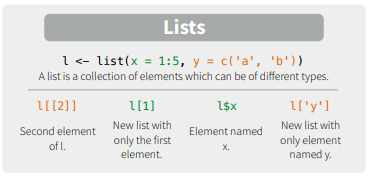
\includegraphics[width=4.16667in,height=\textheight]{images/03/05.PNG}

\begin{Shaded}
\begin{Highlighting}[]
\DocumentationTok{\#\# list}
\NormalTok{parent\_names }\OtherTok{\textless{}{-}} \FunctionTok{c}\NormalTok{(}\StringTok{"Fred"}\NormalTok{, }\StringTok{"Mary"}\NormalTok{)}
\NormalTok{number\_of\_children }\OtherTok{\textless{}{-}} \DecValTok{2}
\NormalTok{child\_ages }\OtherTok{\textless{}{-}} \FunctionTok{c}\NormalTok{(}\DecValTok{4}\NormalTok{, }\DecValTok{7}\NormalTok{, }\DecValTok{9}\NormalTok{)}
\FunctionTok{data.frame}\NormalTok{(parent\_names, number\_of\_children, child\_ages)}
\NormalTok{lst }\OtherTok{\textless{}{-}} \FunctionTok{list}\NormalTok{(parent\_names, number\_of\_children, child\_ages)}
\NormalTok{lst[}\DecValTok{1}\NormalTok{]}
\NormalTok{lst[[}\DecValTok{1}\NormalTok{]]}
\FunctionTok{class}\NormalTok{(lst[}\DecValTok{1}\NormalTok{])}
\FunctionTok{class}\NormalTok{(lst[[}\DecValTok{1}\NormalTok{]])}
\NormalTok{lst[[}\DecValTok{1}\NormalTok{]][}\DecValTok{1}\NormalTok{]}
\NormalTok{lst[[}\DecValTok{1}\NormalTok{]][}\FunctionTok{c}\NormalTok{(}\DecValTok{1}\NormalTok{,}\DecValTok{2}\NormalTok{)]}
\end{Highlighting}
\end{Shaded}

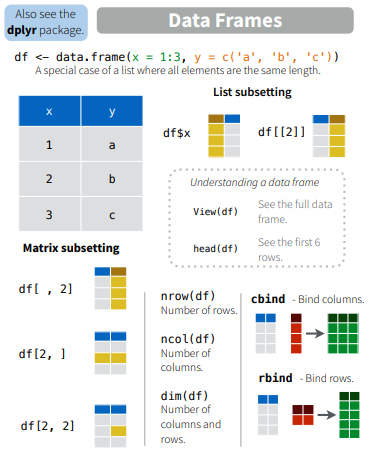
\includegraphics[width=5.20833in,height=\textheight]{images/03/06.PNG}

\hypertarget{a-script-in-r}{%
\section{A script in R}\label{a-script-in-r}}

R 프로그래밍을 통해서 사용자가 원하는 기능을 수행하는 방법은 다음과 같이 스크립트를 만들어서 실행하는 것 입니다. 일반적으로 R을 이용한 스크립트 명령을 어떻게 실행하는지 알아보겠습니다. 다음 예제는 입력 값들의 평균을 계산해서 출력해 주는 스크립트 명령입니다. R base 패키지에서 기본으로 제공되는 \texttt{mean()}이라는 함수가 있지만 사용하지 않고 \texttt{sum()}과 \texttt{length()} 함수를 사용했습니다.

\begin{Shaded}
\begin{Highlighting}[]

\NormalTok{numbers }\OtherTok{\textless{}{-}} \FunctionTok{c}\NormalTok{(}\FloatTok{0.452}\NormalTok{, }\FloatTok{1.474}\NormalTok{, }\FloatTok{0.22}\NormalTok{, }\FloatTok{0.545}\NormalTok{, }\FloatTok{1.205}\NormalTok{, }\FloatTok{3.55}\NormalTok{)}
\FunctionTok{cat}\NormalTok{(}\StringTok{"Input numbers are"}\NormalTok{, numbers, }\StringTok{"}\SpecialCharTok{\textbackslash{}n}\StringTok{"}\NormalTok{)}
\NormalTok{numbers\_mean }\OtherTok{\textless{}{-}} \FunctionTok{sum}\NormalTok{(numbers)}\SpecialCharTok{/}\FunctionTok{length}\NormalTok{(numbers)}
\NormalTok{out }\OtherTok{\textless{}{-}} \FunctionTok{paste}\NormalTok{(}\StringTok{"The average is "}\NormalTok{, numbers\_mean, }\StringTok{".}\SpecialCharTok{\textbackslash{}n}\StringTok{"}\NormalTok{, }\AttributeTok{sep=}\StringTok{""}\NormalTok{)}
\FunctionTok{cat}\NormalTok{(out)}
\end{Highlighting}
\end{Shaded}

상황에 따라 다르긴 하지만 보통 위 스크립트를 실행할 때 R 파일을 하나 만들고 \texttt{source()}라는 함수를 사용해서 파일 전체를 한번에 읽어들이고 실행을 시킵니다. 위 코드를 \texttt{myscript.R} 이라는 새로운 R 파일을 하나 만들고 저장 후 다음과 같이 실행할 수 있습니다. 참고로 위 파일은 현재 Working directory와 같은 위치에 저장해야 합니다.

\begin{Shaded}
\begin{Highlighting}[]
\FunctionTok{source}\NormalTok{(}\StringTok{"myscript.R"}\NormalTok{)}
\end{Highlighting}
\end{Shaded}

그러나 위와 같은 식으로 실행할 경우 다음 몇 가지 문제가 있습니다. 하나는 입력 값이 바뀔 때마나 파일을 열어 바뀐 값을 저장해 줄 필요가 있습니다. 결과 값에 대해서 다른 처리를 하고 싶을 경우 또한 파일을 직접 수정해 주어야 합니다. 또한 모든 변수들이 전역변수로 사용되어 코드가 복잡해질 경우 변수간 간섭이 생길 가능성이 높습니다.

\hypertarget{functions}{%
\section{Functions}\label{functions}}

함수(Function)란 사용자가 원하는 기능을 수행하는 코드의 모음으로서 반복적으로 쉽게 사용할 수 있도록 만들어 놓은 코드 입니다. 특정 데이터를 입력으로 받아 원하는 기능을 수행한 후 결과 데이터를 반환하는 구조를 가집니다. 함수는 일반적으로 다음과 같은 포멧으로 구현할 수 있습니다.

\begin{Shaded}
\begin{Highlighting}[]
\NormalTok{my\_function\_name }\OtherTok{\textless{}{-}} \ControlFlowTok{function}\NormalTok{(parameter1, parameter2, ... )\{}
  \DocumentationTok{\#\#any statements}
  \FunctionTok{return}\NormalTok{(object)}
\NormalTok{\}}
\end{Highlighting}
\end{Shaded}

예를 들어 다음과 같은 \texttt{my\_sine} 함수를 만들 수 있으며 parameter (매개변수)는 \texttt{x}이고 \texttt{y}는 반환값을 저장하는 지역변수 입니다.

\begin{Shaded}
\begin{Highlighting}[]
\NormalTok{my\_sine }\OtherTok{\textless{}{-}} \ControlFlowTok{function}\NormalTok{(x)\{}
\NormalTok{    y }\OtherTok{\textless{}{-}} \FunctionTok{sin}\NormalTok{(x)}
    \FunctionTok{return}\NormalTok{(y)}
\NormalTok{\}}
\end{Highlighting}
\end{Shaded}

만들어진 함수는 다음과 같이 사용할 수 있습니다. 만들어진 함수는 처음에 한 번 실행해 주어 실행중인 R session에 등록한 후 사용할 수 있습니다. 여기서 함수로 전달되는 값 \texttt{pi}는 argument (전달인자) 라고 합니다. 전달인자는 함수에서 정의된 매개변수의 갯수와 같은 수의 전달인자를 입력해 주어야 합니다.

\begin{Shaded}
\begin{Highlighting}[]
\FunctionTok{my\_sine}\NormalTok{(pi)}
\FunctionTok{my\_sine}\NormalTok{(}\DecValTok{90}\NormalTok{)}
\FunctionTok{sin}\NormalTok{(}\DecValTok{90}\NormalTok{)}
\end{Highlighting}
\end{Shaded}

\begin{itemize}
\item
  Terminology

  \begin{itemize}
  \tightlist
  \item
    function name: \texttt{my\_sine}
  \item
    parameter: \texttt{x}
  \item
    argument: \texttt{pi}
  \item
    return value: \texttt{y}
  \end{itemize}
\end{itemize}

이제 위 스크립트 (`myscript.R') 에서 사용된 코드를 함수로 바꿔봅니다. numbers (전달인자)를 받는 매개변수를 x로 하고 함수 이름은 \texttt{mymean} 이고 평균값 (numbers\_mean)을 반환하는 합수입니다.

\begin{Shaded}
\begin{Highlighting}[]
\NormalTok{numbers }\OtherTok{\textless{}{-}} \FunctionTok{c}\NormalTok{(}\FloatTok{0.452}\NormalTok{, }\FloatTok{1.474}\NormalTok{, }\FloatTok{0.22}\NormalTok{, }\FloatTok{0.545}\NormalTok{, }\FloatTok{1.205}\NormalTok{, }\FloatTok{3.55}\NormalTok{)}

\NormalTok{mymean }\OtherTok{\textless{}{-}} \ControlFlowTok{function}\NormalTok{(x)\{}
  \FunctionTok{cat}\NormalTok{(}\StringTok{"Input numbers are"}\NormalTok{, x, }\StringTok{"}\SpecialCharTok{\textbackslash{}n}\StringTok{"}\NormalTok{)}
\NormalTok{  numbers\_mean }\OtherTok{\textless{}{-}} \FunctionTok{sum}\NormalTok{(x)}\SpecialCharTok{/}\FunctionTok{length}\NormalTok{(x)}
\NormalTok{  out }\OtherTok{\textless{}{-}} \FunctionTok{paste}\NormalTok{(}\StringTok{"The average is "}\NormalTok{, numbers\_mean, }\StringTok{".}\SpecialCharTok{\textbackslash{}n}\StringTok{"}\NormalTok{, }\AttributeTok{sep=}\StringTok{""}\NormalTok{)}
  \FunctionTok{cat}\NormalTok{(out)}
  \FunctionTok{return}\NormalTok{(numbers\_mean)}
\NormalTok{\}}

\NormalTok{retval }\OtherTok{\textless{}{-}} \FunctionTok{mymean}\NormalTok{(numbers)}
\FunctionTok{cat}\NormalTok{(retval)}
\end{Highlighting}
\end{Shaded}

\texttt{myscript.R}이라는 파일을 열고 작성된 스크립트에 더해서 아래처럼 함수 코드를 만들 경우 \texttt{source()} 함수로 함수를 세션으로 읽어오고 바로 사용할 수 있습니다. 위와 같이 함수를 만들 경우 입력 값을 언제든 바꿔서 사용할 수 있고 반환값에 대한 추가적인 연산도 쉽게 수행 할 수 있습니다.

\begin{Shaded}
\begin{Highlighting}[]
\NormalTok{new\_values }\OtherTok{\textless{}{-}} \FunctionTok{c}\NormalTok{(}\DecValTok{1}\SpecialCharTok{:}\DecValTok{10}\NormalTok{)}
\NormalTok{retval }\OtherTok{\textless{}{-}} \FunctionTok{mymean}\NormalTok{(new\_values)}
\NormalTok{retval}
\end{Highlighting}
\end{Shaded}

\hypertarget{exercise-7}{%
\subsubsection*{Exercise}\label{exercise-7}}
\addcontentsline{toc}{subsubsection}{Exercise}

\begin{enumerate}
\def\labelenumi{\arabic{enumi}.}
\item
  변수 \texttt{x}에 1, 3, 5, 7, 9를, 변수 \texttt{y}에 2, 4, 6, 8, 10을 저장하는 코드를 작성하시오
\item
  \texttt{x}와 \texttt{y}를 더한 값을 \texttt{z}에 저장하는 코드를 작성하시오
\item
  \texttt{mysum} 이라는 이름의 함수를 작성하되 두 변수를 입력으로 받아 더한 후 결과를 반환하는 코드를 작성하시오
\item
  \texttt{mymean} 이라는 이름의 함수를 작성하되 두 변수를 입력으로 받아 평균을 구한 후 결과를 반환하는 코드를 작성하시오
\end{enumerate}

\hypertarget{exercise-8}{%
\subsubsection*{Exercise}\label{exercise-8}}
\addcontentsline{toc}{subsubsection}{Exercise}

\begin{enumerate}
\def\labelenumi{\arabic{enumi})}
\tightlist
\item
  \texttt{mysd}라는 이름의 (표본)표준편차를 구하는 함수를 \texttt{myscript.R} 파일에 구현하시오 (\texttt{sd()}함수 사용하지 않고, 다음 표준편차 공식 이용)
\end{enumerate}

\[ 
\sigma = \sqrt{\frac{\sum(x-mean(x))^2}{length(x)-1}} 
\]

코드는 아래와 같음

\begin{Shaded}
\begin{Highlighting}[]
\NormalTok{mysd }\OtherTok{\textless{}{-}} \ControlFlowTok{function}\NormalTok{(x)\{}
\NormalTok{  numbers\_sd }\OtherTok{\textless{}{-}} \FunctionTok{sqrt}\NormalTok{(}\FunctionTok{sum}\NormalTok{((x }\SpecialCharTok{{-}} \FunctionTok{mymean}\NormalTok{(x))}\SpecialCharTok{\^{}}\DecValTok{2}\NormalTok{)}\SpecialCharTok{/}\NormalTok{(}\FunctionTok{length}\NormalTok{(x)}\SpecialCharTok{{-}}\DecValTok{1}\NormalTok{))  }
  \FunctionTok{return}\NormalTok{(numbers\_sd)}
\NormalTok{\}}
\end{Highlighting}
\end{Shaded}

\begin{enumerate}
\def\labelenumi{\arabic{enumi})}
\setcounter{enumi}{1}
\tightlist
\item
  1부터 100까지의 값을 \texttt{x}에 저장하고 mysd 함수를 사용해서 표준편차를 구하시오
\end{enumerate}

\begin{Shaded}
\begin{Highlighting}[]
\NormalTok{x }\OtherTok{\textless{}{-}} \DecValTok{1}\SpecialCharTok{:}\DecValTok{100}
\FunctionTok{mysd}\NormalTok{(x)}
\end{Highlighting}
\end{Shaded}

\begin{enumerate}
\def\labelenumi{\arabic{enumi})}
\setcounter{enumi}{2}
\tightlist
\item
  앞서 작성한 \texttt{mymean} 함수와 \texttt{mysd} 함수를 같이 사용하여 \texttt{x}를 표준화 하고 \texttt{z}로 저장하시오. 표준화 공식은 다음과 같음
\end{enumerate}

\[ 
z = \frac{x - mean(x)}{sd(x)}
\]

\begin{Shaded}
\begin{Highlighting}[]
\NormalTok{z }\OtherTok{\textless{}{-}}\NormalTok{ (x }\SpecialCharTok{{-}} \FunctionTok{mymean}\NormalTok{(x))}\SpecialCharTok{/}\FunctionTok{mysd}\NormalTok{(x)}
\end{Highlighting}
\end{Shaded}

\begin{enumerate}
\def\labelenumi{\arabic{enumi})}
\setcounter{enumi}{3}
\tightlist
\item
  \texttt{x} 와 \texttt{z}를 갖는 \texttt{y}라는 이름의 \texttt{data.frame}을 생성하시오
\end{enumerate}

\hypertarget{local-and-global-variables}{%
\subsection{local and global variables}\label{local-and-global-variables}}

다음 코드를 보면 전역변수 \texttt{x}, \texttt{y}는 지역변수 \texttt{x}, \texttt{y}와 독립적으로 사용됨을 알 수 있습니다.

\begin{Shaded}
\begin{Highlighting}[]
\NormalTok{my\_half }\OtherTok{\textless{}{-}} \ControlFlowTok{function}\NormalTok{(x)\{}
\NormalTok{  y }\OtherTok{\textless{}{-}}\NormalTok{ x}\SpecialCharTok{/}\NormalTok{z}
  \FunctionTok{cat}\NormalTok{(}\StringTok{"local variable x:"}\NormalTok{, x, }\StringTok{"}\SpecialCharTok{\textbackslash{}n}\StringTok{"}\NormalTok{)}
  \FunctionTok{cat}\NormalTok{(}\StringTok{"local variable y:"}\NormalTok{, y, }\StringTok{"}\SpecialCharTok{\textbackslash{}n}\StringTok{"}\NormalTok{)}
  \FunctionTok{cat}\NormalTok{(}\StringTok{"global variable z:"}\NormalTok{, z, }\StringTok{"}\SpecialCharTok{\textbackslash{}n}\StringTok{"}\NormalTok{)}
  \FunctionTok{return}\NormalTok{(y)}
\NormalTok{\}}
\NormalTok{y }\OtherTok{\textless{}{-}} \DecValTok{100}
\NormalTok{x }\OtherTok{\textless{}{-}} \DecValTok{20}
\NormalTok{z }\OtherTok{\textless{}{-}} \DecValTok{30}
\FunctionTok{cat}\NormalTok{(}\StringTok{"Global variable x:"}\NormalTok{, x, }\StringTok{"}\SpecialCharTok{\textbackslash{}n}\StringTok{"}\NormalTok{)}
\FunctionTok{cat}\NormalTok{(}\StringTok{"Global variable y:"}\NormalTok{, y, }\StringTok{"}\SpecialCharTok{\textbackslash{}n}\StringTok{"}\NormalTok{)}
\FunctionTok{cat}\NormalTok{(}\StringTok{"Global variable z:"}\NormalTok{, z, }\StringTok{"}\SpecialCharTok{\textbackslash{}n}\StringTok{"}\NormalTok{)}
\FunctionTok{my\_half}\NormalTok{(}\DecValTok{5}\NormalTok{)}

\NormalTok{my\_half }\OtherTok{\textless{}{-}} \ControlFlowTok{function}\NormalTok{(x, z)\{}
\NormalTok{  y }\OtherTok{\textless{}{-}}\NormalTok{ x}\SpecialCharTok{/}\NormalTok{z}
  \FunctionTok{cat}\NormalTok{(}\StringTok{"local variable x:"}\NormalTok{, x, }\StringTok{"}\SpecialCharTok{\textbackslash{}n}\StringTok{"}\NormalTok{)}
  \FunctionTok{cat}\NormalTok{(}\StringTok{"local variable y:"}\NormalTok{, y, }\StringTok{"}\SpecialCharTok{\textbackslash{}n}\StringTok{"}\NormalTok{)}
  \FunctionTok{cat}\NormalTok{(}\StringTok{"local variable z:"}\NormalTok{, z, }\StringTok{"}\SpecialCharTok{\textbackslash{}n}\StringTok{"}\NormalTok{)}
  \FunctionTok{return}\NormalTok{(y)}
\NormalTok{\}}

\FunctionTok{my\_half}\NormalTok{(}\DecValTok{5}\NormalTok{, }\DecValTok{10}\NormalTok{)}
\end{Highlighting}
\end{Shaded}

\texttt{log}, \texttt{sin}등의 함수들은 Built-in function으로 같은 이름의 함수를 만들지 않도록 주의합니다.

\begin{Shaded}
\begin{Highlighting}[]
\NormalTok{x }\OtherTok{\textless{}{-}}\NormalTok{ pi}
\FunctionTok{sin}\NormalTok{(x)}
\FunctionTok{sqrt}\NormalTok{(x)}
\FunctionTok{log}\NormalTok{(x)}
\FunctionTok{log}\NormalTok{(x, }\DecValTok{10}\NormalTok{)}
\NormalTok{x }\OtherTok{\textless{}{-}} \FunctionTok{c}\NormalTok{(}\DecValTok{10}\NormalTok{, }\DecValTok{20}\NormalTok{, }\DecValTok{30}\NormalTok{)}
\NormalTok{x }\SpecialCharTok{+}\NormalTok{ x}
\FunctionTok{mean}\NormalTok{(x)}
\FunctionTok{sum}\NormalTok{(x)}\SpecialCharTok{/}\FunctionTok{length}\NormalTok{(x)}
\end{Highlighting}
\end{Shaded}

\hypertarget{vectorized-functions}{%
\subsection{Vectorized functions}\label{vectorized-functions}}

초기에 R이 다른 프로그래밍 언어에 비해서 경쟁력을 갖는 이유 중 하나가 바로 이 벡터 연산 기능 이였습니다. \texttt{vector} 변수에 들어있는 각 원소들에 대해서 특정 함수나 연산을 적용하고 싶을 경우 전통 방식의 \texttt{C}나 \texttt{Java}등의 언어에서는 원소의 개수만큼 반복문을 돌면서 원하는 작업을 수행 했습니다. 그러나 R의 벡터 연산 기능은 별도의 반복문 없이 vector 안에 있는 원소들에 대한 함수 실행 또는 연산을 수행할 수 있습니다.

\begin{Shaded}
\begin{Highlighting}[]
\NormalTok{x }\OtherTok{\textless{}{-}} \FunctionTok{c}\NormalTok{(}\DecValTok{10}\NormalTok{, }\DecValTok{20}\NormalTok{, }\DecValTok{30}\NormalTok{)}
\NormalTok{x }\SpecialCharTok{+}\NormalTok{ x}
\FunctionTok{sqrt}\NormalTok{(x)}
\FunctionTok{sin}\NormalTok{(x)}
\FunctionTok{log}\NormalTok{(x)}
\NormalTok{x}\SpecialCharTok{{-}}\FunctionTok{mean}\NormalTok{(x)}

\FunctionTok{length}\NormalTok{(x)}
\NormalTok{test\_scores }\OtherTok{\textless{}{-}} \FunctionTok{c}\NormalTok{(}\AttributeTok{Alice =} \DecValTok{87}\NormalTok{, }\AttributeTok{Bob =} \DecValTok{72}\NormalTok{, }\AttributeTok{James=} \DecValTok{99}\NormalTok{)}
\FunctionTok{names}\NormalTok{(test\_scores)}
\end{Highlighting}
\end{Shaded}

\hypertarget{exercise-9}{%
\subsubsection*{Exercise}\label{exercise-9}}
\addcontentsline{toc}{subsubsection}{Exercise}

다음은 한 다이어트 프로그램의 수행 전 후의 다섯 명의 몸무게이다.

\begin{longtable}[]{@{}llllll@{}}
\toprule()
\endhead
Before & 78 & 72 & 78 & 79 & 105 \\
after & 67 & 65 & 79 & 70 & 93 \\
\bottomrule()
\end{longtable}

\begin{enumerate}
\def\labelenumi{\arabic{enumi})}
\item
  각각을 before 와 after 이름의 변수에 저장 후 몸무게 값의 변화량을 계산하여 diff 라는 변수에 저장하시오
\item
  diff에 저장된 값들의 합, 평균, 표준편차를 구하시오
\end{enumerate}

\hypertarget{exercise-10}{%
\subsubsection*{Exercise}\label{exercise-10}}
\addcontentsline{toc}{subsubsection}{Exercise}

다음 네 학생이 있으며 ``John'',``James'',``Sara'', ``Lilly'' 각 나이는 21, 55, 23, 53 이다. ages 라는 변수를 생성하고 각 나이를 저장한 후 who라는 이름의 함수를 만들어서 50살 이상인 사람의 이름을 출력하는 함수를 만드시오.

\begin{itemize}
\tightlist
\item
  \texttt{ages}라는 변수에 나이 저장, c() 함수 이용, vector 형태 저장
\item
  names() 함수 이용해서 각 \texttt{ages} 벡터의 각 요소에 이름 붙이기
\item
  which() 함수 사용해서 나이가 50보다 큰 인덱스 찾고 해당 인덱스 값들을 \texttt{idx}에 저장
\item
  \texttt{ages}에서 \texttt{idx}에 해당하는 인덱스를 갖는 값을 \texttt{sel\_ages}에 저장
\item
  \texttt{names()}함수를 이용해서 \texttt{sel\_ages}의 이름을 \texttt{sel\_names}에 저장
\item
  위 설명을 참고해서 \texttt{input}이라는 파라메터를 갖고 \texttt{sel\_names}라는 50살 이상인 사람의 이름을 반환하는 \texttt{who50}이라는 이름의 함수 만들기
\item
  \texttt{who50} 함수의 사용법은 \texttt{who50(ages)} 임
\end{itemize}

\hypertarget{flow-control}{%
\section{Flow control}\label{flow-control}}

\hypertarget{if-statements}{%
\subsection{if statements}\label{if-statements}}

R에서의 제어문의 사용은 다른 프로그래밍 언어와 거의 유사합니다. 먼저 \texttt{if} 는 다음과 같은 형식으로 사용되며 \texttt{()} 안에 특정 조건 판단을 위한 표현이 들어갑니다.

\begin{Shaded}
\begin{Highlighting}[]
\ControlFlowTok{if}\NormalTok{(condition)\{}
\NormalTok{  expr\_1}
\NormalTok{\}}\ControlFlowTok{else}\NormalTok{\{}
\NormalTok{  expr\_2}
\NormalTok{\}}
\end{Highlighting}
\end{Shaded}

특히 \texttt{condition}은 하나의 원소에 대한 조건 판단문으로 \texttt{T} 또는 \texttt{F} 값 하나만을 반환하는 문장이어야 합니다. 위 코드는 만약 \texttt{condition} 조건이 \texttt{True} 이면 expr\_1를 실행하고 \texttt{False}이면 expr\_2를 실행하라는 명령입니다. \texttt{condition} 안에서 사용되는 비교 연산자들은 다음과 같습니다.

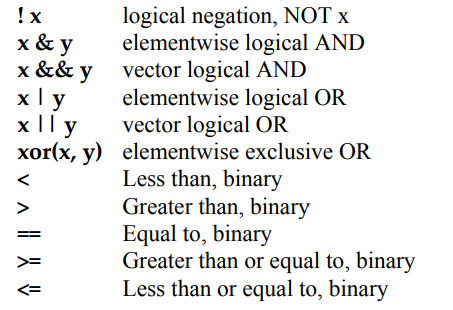
\includegraphics{images/04/01.PNG}

\begin{Shaded}
\begin{Highlighting}[]
\NormalTok{x }\OtherTok{\textless{}{-}} \DecValTok{2}
\ControlFlowTok{if}\NormalTok{(x}\SpecialCharTok{\%\%}\DecValTok{2} \SpecialCharTok{==} \DecValTok{1}\NormalTok{)\{}
  \FunctionTok{cat}\NormalTok{(}\StringTok{"Odd"}\NormalTok{)}
\NormalTok{\}}\ControlFlowTok{else}\NormalTok{\{}
  \FunctionTok{cat}\NormalTok{(}\StringTok{"Even"}\NormalTok{)}
\NormalTok{\} }

\NormalTok{x }\OtherTok{\textless{}{-}} \DecValTok{5}
\ControlFlowTok{if}\NormalTok{(x }\SpecialCharTok{\textgreater{}} \DecValTok{0} \SpecialCharTok{\&}\NormalTok{ x }\SpecialCharTok{\textless{}} \DecValTok{4}\NormalTok{)\{}
  \FunctionTok{print}\NormalTok{(}\StringTok{"Positive number less than four"}\NormalTok{)}
\NormalTok{\}}

\ControlFlowTok{if}\NormalTok{(x }\SpecialCharTok{\textgreater{}} \DecValTok{0}\NormalTok{) }\FunctionTok{print}\NormalTok{(}\StringTok{"Positive number"}\NormalTok{)}

\NormalTok{x }\OtherTok{\textless{}{-}} \SpecialCharTok{{-}}\DecValTok{5}
\ControlFlowTok{if}\NormalTok{(x }\SpecialCharTok{\textgreater{}} \DecValTok{0}\NormalTok{)\{}
  \FunctionTok{print}\NormalTok{(}\StringTok{"Non{-}negative number"}\NormalTok{)}
\NormalTok{\} }\ControlFlowTok{else} \ControlFlowTok{if}\NormalTok{(x }\SpecialCharTok{\textless{}=} \DecValTok{0} \SpecialCharTok{\&}\NormalTok{ x }\SpecialCharTok{\textgreater{}} \SpecialCharTok{{-}}\DecValTok{5}\NormalTok{)\{}
  \FunctionTok{print}\NormalTok{(}\StringTok{"Negative number greater than {-}5"}\NormalTok{)}
\NormalTok{\} }\ControlFlowTok{else}\NormalTok{ \{}
  \FunctionTok{print}\NormalTok{(}\StringTok{"Negative number less than {-}5"}\NormalTok{)}
\NormalTok{\}}

\ControlFlowTok{if}\NormalTok{(x }\SpecialCharTok{\textgreater{}} \DecValTok{0}\NormalTok{)}
  \FunctionTok{print}\NormalTok{(}\StringTok{"Non{-}negative number"}\NormalTok{)}
\ControlFlowTok{else}
  \FunctionTok{print}\NormalTok{(}\StringTok{"Negative number"}\NormalTok{)}
\end{Highlighting}
\end{Shaded}

\hypertarget{ifelse-statements}{%
\section{ifelse statements}\label{ifelse-statements}}

\texttt{if}는 하나의 조건만 비교하는데 사용할 수 있습니다. 그러나 변수에는 여러 값이 벡터형식으로 들어가고 벡터연산을 수행할 경우의 결과도 벡터형식으로 나오지만 \texttt{if}문은 이들을 한 번에 처리하기 어렵습니다. \texttt{ifelse}는 이러한 단점을 보완하여 여러 값을 한번에 처리할 수 있습니다.

\begin{Shaded}
\begin{Highlighting}[]
\FunctionTok{ifelse}\NormalTok{ (condition, True일 때 리턴값, False일 때 리턴값)}
\end{Highlighting}
\end{Shaded}

\begin{Shaded}
\begin{Highlighting}[]

\NormalTok{x }\OtherTok{\textless{}{-}} \FunctionTok{c}\NormalTok{(}\DecValTok{1}\SpecialCharTok{:}\DecValTok{10}\NormalTok{)}
\ControlFlowTok{if}\NormalTok{(x}\SpecialCharTok{\textgreater{}}\DecValTok{10}\NormalTok{)\{}
  \FunctionTok{cat}\NormalTok{(}\StringTok{"Big"}\NormalTok{)}
\NormalTok{\}}\ControlFlowTok{else}\NormalTok{\{}
  \FunctionTok{cat}\NormalTok{(}\StringTok{"Small"}\NormalTok{)}
\NormalTok{\}}

\FunctionTok{ifelse}\NormalTok{(x}\SpecialCharTok{\textgreater{}}\DecValTok{10}\NormalTok{, }\StringTok{"Big"}\NormalTok{, }\StringTok{"Small"}\NormalTok{)}
\end{Highlighting}
\end{Shaded}

그러나 출력만 가능하며 조건별로 다른 명령 수행은 불가능하다는 단점이 있습니다.

\hypertarget{exercise-11}{%
\subsubsection*{Exercise}\label{exercise-11}}
\addcontentsline{toc}{subsubsection}{Exercise}

다음은 median (중간값)을 구하는 공식이며 x의 길이가 (n이) 홀수일 경우와 짝수일 경우에 따라서 다른 공식이 사용된다. 다음 공식과 코드를 이용하여 mymedian 이라는 이름의 함수를 만들고 입력 값들의 중간값을 구해서 반환하는 함수를 만드시오. (\texttt{\%\%} 나머지 연산, \texttt{if}문 사용, 아래 중간값 코드 참고)

\[
median(X) =
\begin{cases}
\frac{1}{2} X[\frac{n}{2}] + \frac{1}{2} X[1+\frac{n}{2}] & \mbox{if } n \mbox{ is even} \\
X[\frac{n+1}{2}] & \mbox{if } n \mbox{ is odd}
\end{cases}
\]

\begin{Shaded}
\begin{Highlighting}[]
\NormalTok{sorted\_x }\OtherTok{\textless{}{-}} \FunctionTok{sort}\NormalTok{(x)}
\CommentTok{\# 만약 짝수이면 }
\NormalTok{retval }\OtherTok{\textless{}{-}}\NormalTok{ sort\_x[n}\SpecialCharTok{/}\DecValTok{2}\NormalTok{]}\SpecialCharTok{/}\DecValTok{2} \SpecialCharTok{+}\NormalTok{ sort\_x[}\DecValTok{1}\SpecialCharTok{+}\NormalTok{(n}\SpecialCharTok{/}\DecValTok{2}\NormalTok{)]}\SpecialCharTok{/}\DecValTok{2}
\CommentTok{\# 만약 홀수이면 }
\NormalTok{retval }\OtherTok{\textless{}{-}}\NormalTok{ sort\_x[(n}\SpecialCharTok{+}\DecValTok{1}\NormalTok{)}\SpecialCharTok{/}\DecValTok{2}\NormalTok{]}
\end{Highlighting}
\end{Shaded}

\hypertarget{for-while-repeat}{%
\section{for, while, repeat}\label{for-while-repeat}}

\texttt{for} 문은 반복적으로 특정 코드를 실행하고자 할 때 사용됩니다. 다음과 같은 형식으로 사용할 수 있습니다.

\begin{Shaded}
\begin{Highlighting}[]
\ControlFlowTok{for}\NormalTok{(var }\ControlFlowTok{in}\NormalTok{ seq)\{}
\NormalTok{  expression}
\NormalTok{\}}
\end{Highlighting}
\end{Shaded}

\texttt{var}는 반복을 돌 때마다 바뀌는 변수로 \texttt{\{\}} 안에서 사용되는 지역 변수 입니다. \texttt{seq}는 vector 형식의 변수로 반복을 돌 때마다 순차적으로 \texttt{var}에 저장되는 값들 입니다.

\begin{Shaded}
\begin{Highlighting}[]
\NormalTok{x }\OtherTok{\textless{}{-}} \DecValTok{1}\SpecialCharTok{:}\DecValTok{10}
\ControlFlowTok{for}\NormalTok{(i }\ControlFlowTok{in}\NormalTok{ x)\{}
  \FunctionTok{cat}\NormalTok{(i, }\StringTok{"}\SpecialCharTok{\textbackslash{}n}\StringTok{"}\NormalTok{)}
  \FunctionTok{flush.console}\NormalTok{()}
\NormalTok{\}}

\NormalTok{sum\_of\_i }\OtherTok{\textless{}{-}} \DecValTok{0}
\ControlFlowTok{for}\NormalTok{(i }\ControlFlowTok{in} \DecValTok{1}\SpecialCharTok{:}\DecValTok{10}\NormalTok{)\{}
\NormalTok{  sum\_of\_i }\OtherTok{\textless{}{-}}\NormalTok{ sum\_of\_i }\SpecialCharTok{+}\NormalTok{ i}
  \FunctionTok{cat}\NormalTok{(i, }\StringTok{" "}\NormalTok{, sum\_of\_i, }\StringTok{"}\SpecialCharTok{\textbackslash{}n}\StringTok{"}\NormalTok{);}\FunctionTok{flush.console}\NormalTok{()}
\NormalTok{\}}
\end{Highlighting}
\end{Shaded}

\texttt{while}문도 \texttt{for}문과 같이 반복적으로 특정 코드를 수행하고자 할 때 사용합니다. 사용하는 문법은 다음과 같으며 \texttt{cond}는 \texttt{True} 또는 \texttt{False} 로 반환되는 조건문을 넣고 \texttt{True} 일 경우 계속해서 반복하면서 \texttt{expressions}를 수행하며 이 반복은 \texttt{cond}가 \texttt{False}로 될 때 까지 계속됩니다.

\begin{Shaded}
\begin{Highlighting}[]
\ControlFlowTok{while}\NormalTok{(cond)\{}
\NormalTok{  expression}
\NormalTok{\}}
\end{Highlighting}
\end{Shaded}

\texttt{while}문을 사용할 경우 다음과 같이 \texttt{indicator}라 불리우는 변수를 하나 정해서 반복 할 때마다 값이 바뀌도록 해 주어야 합니다. 그렇지 않으면 무한 루프를 돌게 되는 문제가 발생합니다.

\begin{Shaded}
\begin{Highlighting}[]
\NormalTok{i }\OtherTok{\textless{}{-}} \DecValTok{10}
\NormalTok{f }\OtherTok{\textless{}{-}} \DecValTok{1}
\ControlFlowTok{while}\NormalTok{(i}\SpecialCharTok{\textgreater{}}\DecValTok{1}\NormalTok{)\{}
\NormalTok{  f }\OtherTok{\textless{}{-}}\NormalTok{ i}\SpecialCharTok{*}\NormalTok{f}
\NormalTok{  i }\OtherTok{\textless{}{-}}\NormalTok{ i}\DecValTok{{-}1}
  \FunctionTok{cat}\NormalTok{(i, f, }\StringTok{"}\SpecialCharTok{\textbackslash{}n}\StringTok{"}\NormalTok{)}
\NormalTok{\}}
\NormalTok{f}
\FunctionTok{factorial}\NormalTok{(}\DecValTok{10}\NormalTok{)}
\end{Highlighting}
\end{Shaded}

\texttt{repeat} 명령은 조건 없이 블럭 안에 있는 코드를 무조건 반복하라는 명령 입니다. 따라서 블럭 중간에 멈추기 위한 코드가 필요하고 이 명령이 \texttt{break} 입니다.

\begin{Shaded}
\begin{Highlighting}[]
\ControlFlowTok{repeat}\NormalTok{\{}
\NormalTok{  expressions}
  \ControlFlowTok{if}\NormalTok{(cond) }\ControlFlowTok{break}
\NormalTok{\}}

\NormalTok{i }\OtherTok{\textless{}{-}} \DecValTok{10}
\NormalTok{f }\OtherTok{\textless{}{-}} \DecValTok{1}
\ControlFlowTok{repeat}\NormalTok{ \{}
\NormalTok{  f }\OtherTok{\textless{}{-}}\NormalTok{ i}\SpecialCharTok{*}\NormalTok{f}
\NormalTok{  i }\OtherTok{\textless{}{-}}\NormalTok{ i}\DecValTok{{-}1}
  \FunctionTok{cat}\NormalTok{(i, f, }\StringTok{"}\SpecialCharTok{\textbackslash{}n}\StringTok{"}\NormalTok{)}
  \ControlFlowTok{if}\NormalTok{(i}\SpecialCharTok{\textless{}}\DecValTok{1}\NormalTok{) }\ControlFlowTok{break}
\NormalTok{\}}
\NormalTok{f}
\FunctionTok{factorial}\NormalTok{(}\DecValTok{10}\NormalTok{)}
\end{Highlighting}
\end{Shaded}

\hypertarget{avoiding-loops}{%
\section{Avoiding Loops}\label{avoiding-loops}}

R에서는 가능하면 loop문을 사용하지 않는 것이 좋습니다. 이는 다른 언어들 보다 반복문이 느리게 수행된다는 이유 때문이기도 합니다. 그러나 R에서는 반복문을 수행하는 것 보다 훨씬 더 빠르게 반복문을 수행 한 것과 같은 결과를 얻을 수 있는 다양한 방법들이 제공되고 있습니다. 차차 그런 기법들에 대한 학습을 진행하도록 하겠습니다.

\begin{Shaded}
\begin{Highlighting}[]
\NormalTok{x }\OtherTok{\textless{}{-}} \DecValTok{1}\SpecialCharTok{:}\FloatTok{1E7}
\FunctionTok{sum}\NormalTok{(x)}
\FunctionTok{system.time}\NormalTok{(}\FunctionTok{sum}\NormalTok{(x))}

\NormalTok{st }\OtherTok{\textless{}{-}} \FunctionTok{proc.time}\NormalTok{()}
\NormalTok{total }\OtherTok{\textless{}{-}} \DecValTok{0}
\ControlFlowTok{for}\NormalTok{(i }\ControlFlowTok{in} \DecValTok{1}\SpecialCharTok{:}\FunctionTok{length}\NormalTok{(x))\{}
\NormalTok{  total }\OtherTok{\textless{}{-}}\NormalTok{ total }\SpecialCharTok{+}\NormalTok{ x[i]}
\NormalTok{\}}
\NormalTok{ed }\OtherTok{\textless{}{-}} \FunctionTok{proc.time}\NormalTok{()}
\NormalTok{ed}\SpecialCharTok{{-}}\NormalTok{st}
\end{Highlighting}
\end{Shaded}

\hypertarget{object-oriented-programming-advanced}{%
\section{Object Oriented Programming (Advanced)}\label{object-oriented-programming-advanced}}

OOP는 객체지향 프로그래밍 이라고 합니다. OOP를 이용해서 프로그래밍으로 풀고자 하는 문제를 좀 더 명확하게 개념을 수립하고 복잡한 코드를 명료하게 만들 수 있습니다. 그런데 R에서 OOP는 다른 언어보다는 좀 더 어려운 개념적인 이해가 필요합니다. \texttt{S3}, \texttt{S4}, 그리고 \texttt{Reference\ class} 가 있으며 \texttt{S3}, \texttt{S4}는 \texttt{Generic\ function}을 이용하며 다른 언어에서 사용하는 OOP 개념과는 다릅니다. \texttt{Reference\ class}는 다른 언어에서 사용하는 OOP 개념과 유사하며 \texttt{R6} 패키지를 이용해서 사용할 수 있습니다.

\begin{center}\rule{0.5\linewidth}{0.5pt}\end{center}

이 저작물은 크리에이티브 커먼즈 저작자표시-비영리-변경금지 4.0 국제 라이선스에 따라 이용할 수 있습니다.

  \bibliography{book.bib,packages.bib}

\end{document}
